\subsection{Gradient decent methods}


\begin{figure}[H]
\centering
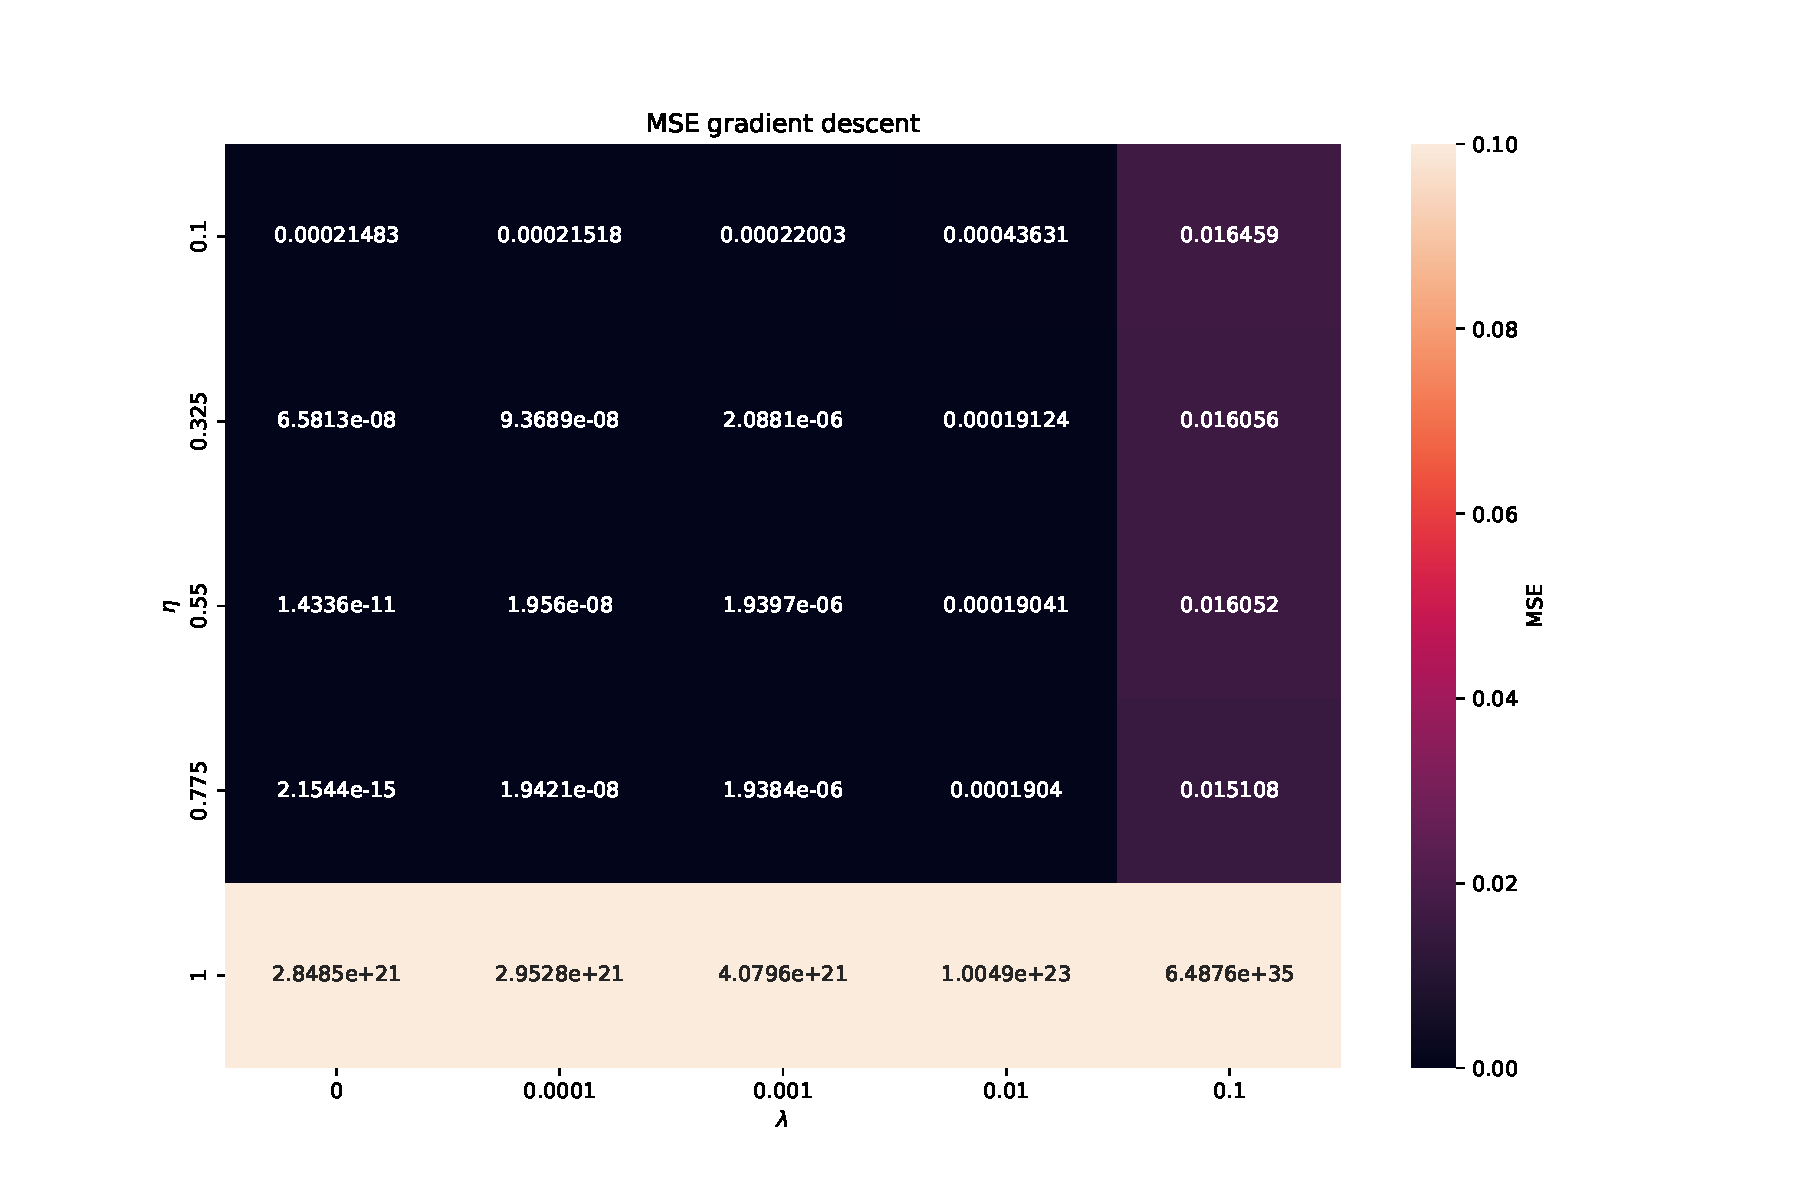
\includegraphics[width=0.8\textwidth]{Figures/PartA/gd_MSE(eta,lmb)}
\caption{Plain gradient descent: test MSE as a function of \(\eta \) and \(\lambda \). 
The parameters utilized are shown in table \ref{tab:GD_parameters_run_1_2} under run 1.}
\label{fig:gd_MSE-eta-lmb-}
\end{figure}

\begin{figure}[H]
\centering
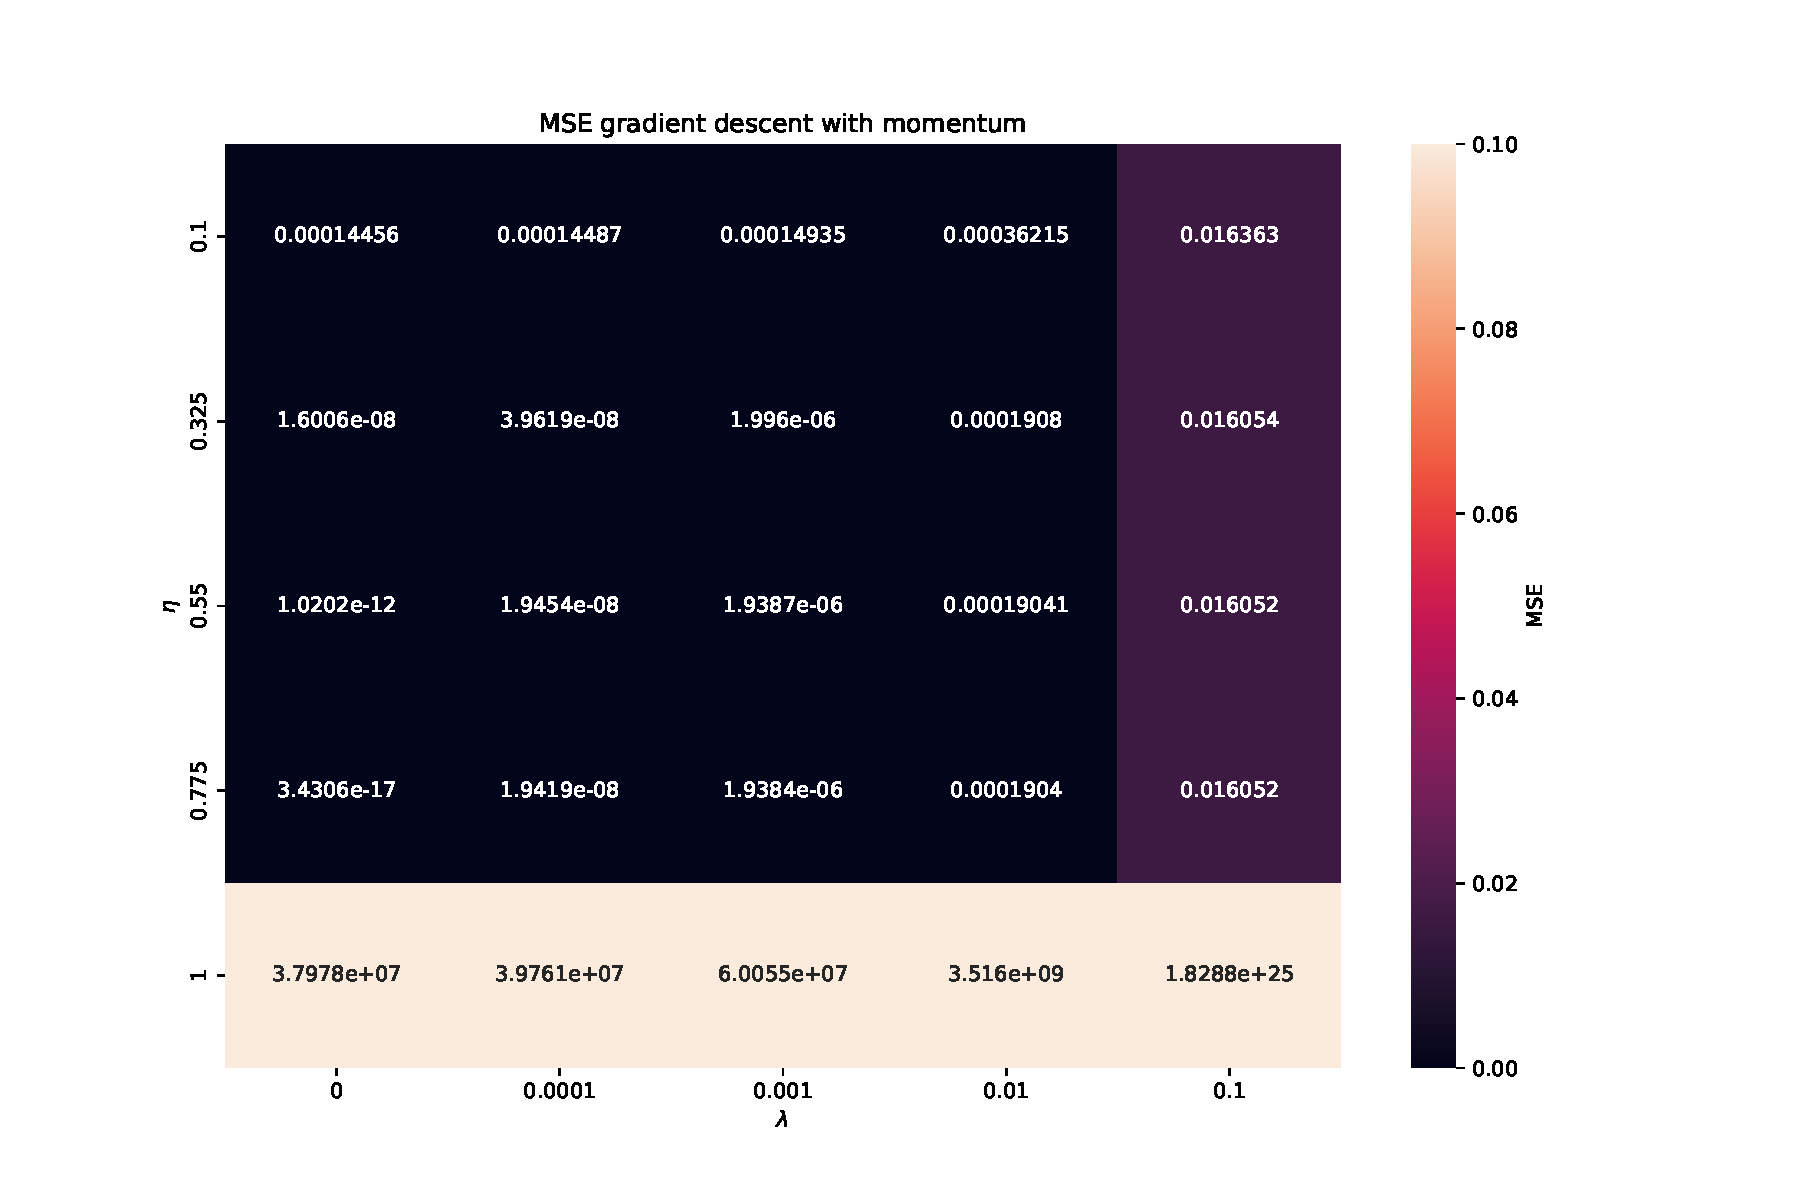
\includegraphics[width=0.8\textwidth]{Figures/PartA/gdm_MSE(eta,lmb)}
\caption{Gradient descent with momentum: test MSE as a function of \(\eta \) and \(\lambda \).
 The parameters utilized are shown in table \ref{tab:GD_parameters_run_1_2} under run 1.}
\label{fig:gdm_MSE-eta-lmb-}
\end{figure}

\begin{figure}[H]
\centering
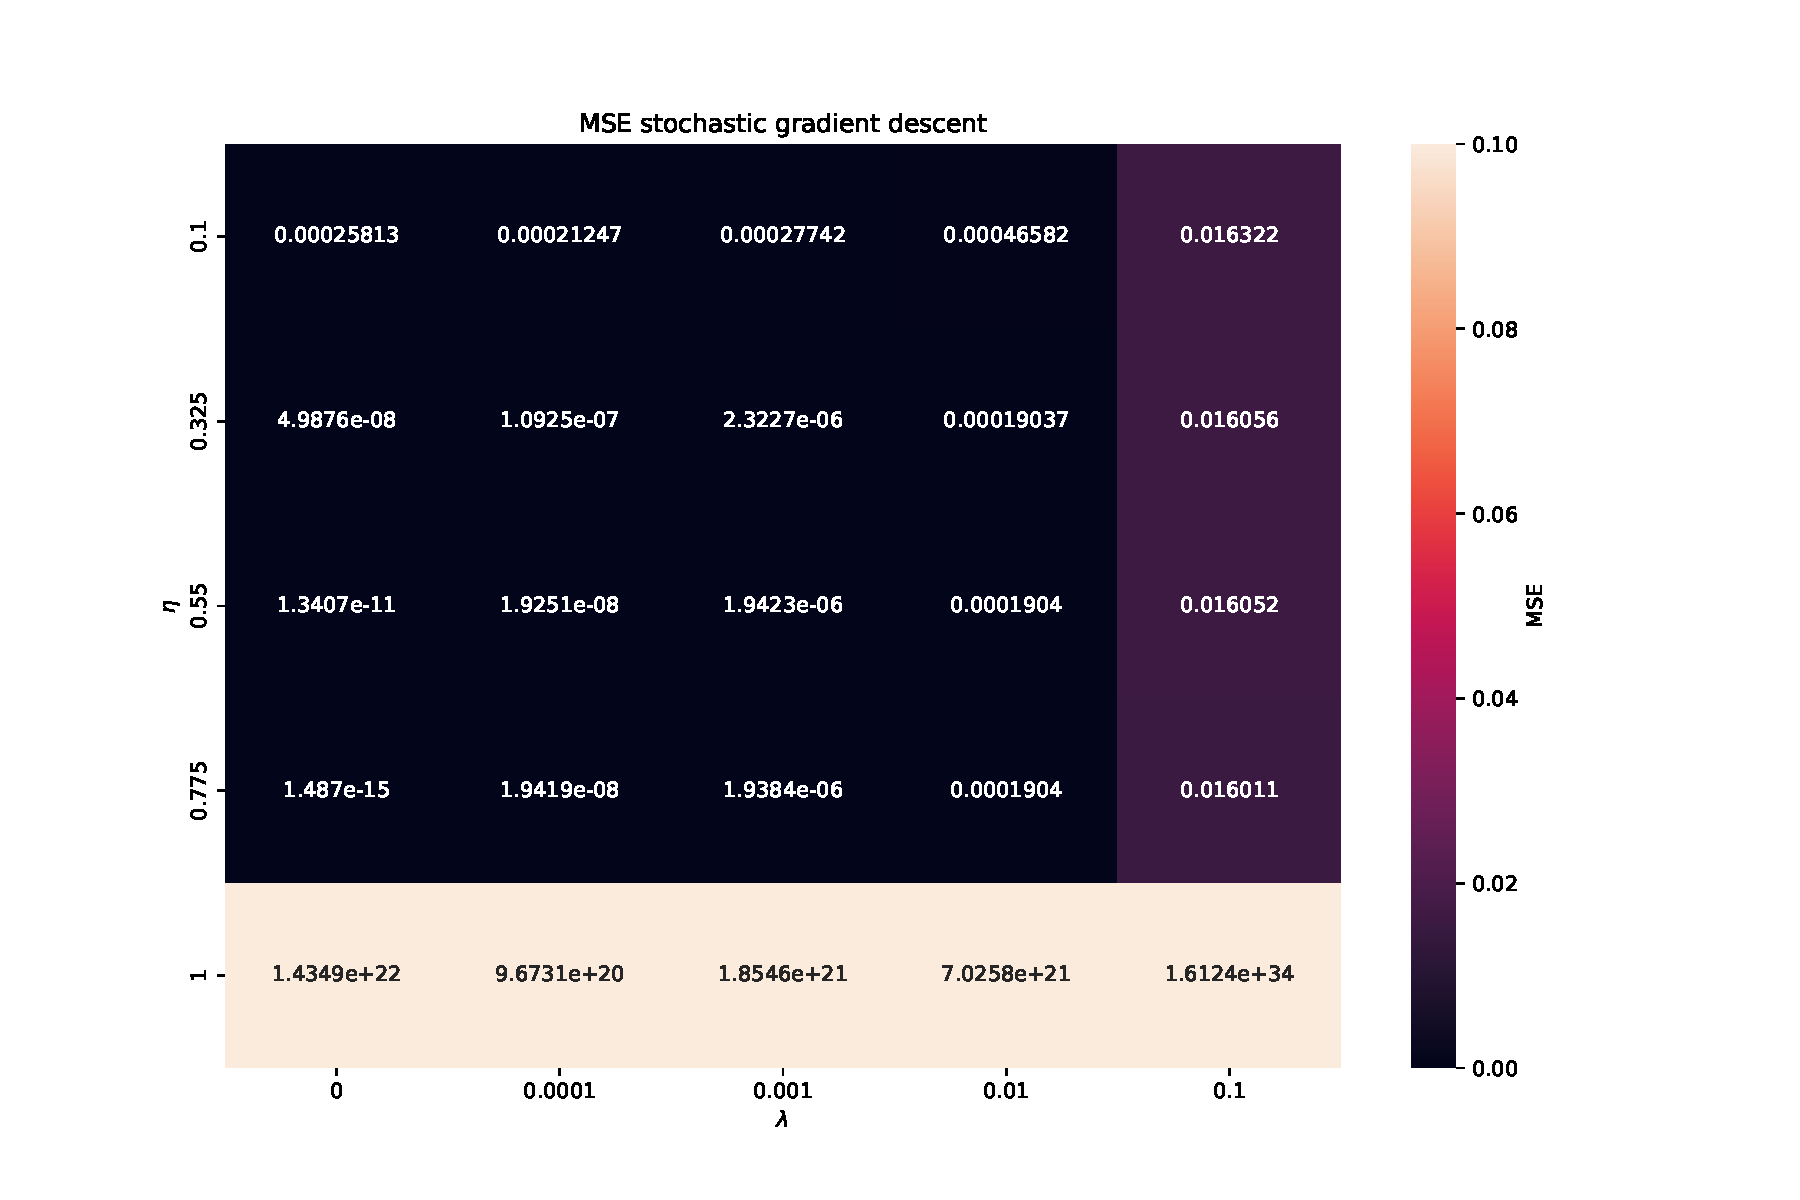
\includegraphics[width=0.8\textwidth]{Figures/PartA/sgd_MSE(eta,lmb)}
\caption{Plain stochastic gradient descent: test MSE as a function of \(\eta \) and \(\lambda \).
 The parameters utilized are shown in table \ref{tab:GD_parameters_run_1_2} under run 1.}
\label{fig:sgd_MSE-eta-lmb-}
\end{figure}

\begin{figure}[H]
\centering
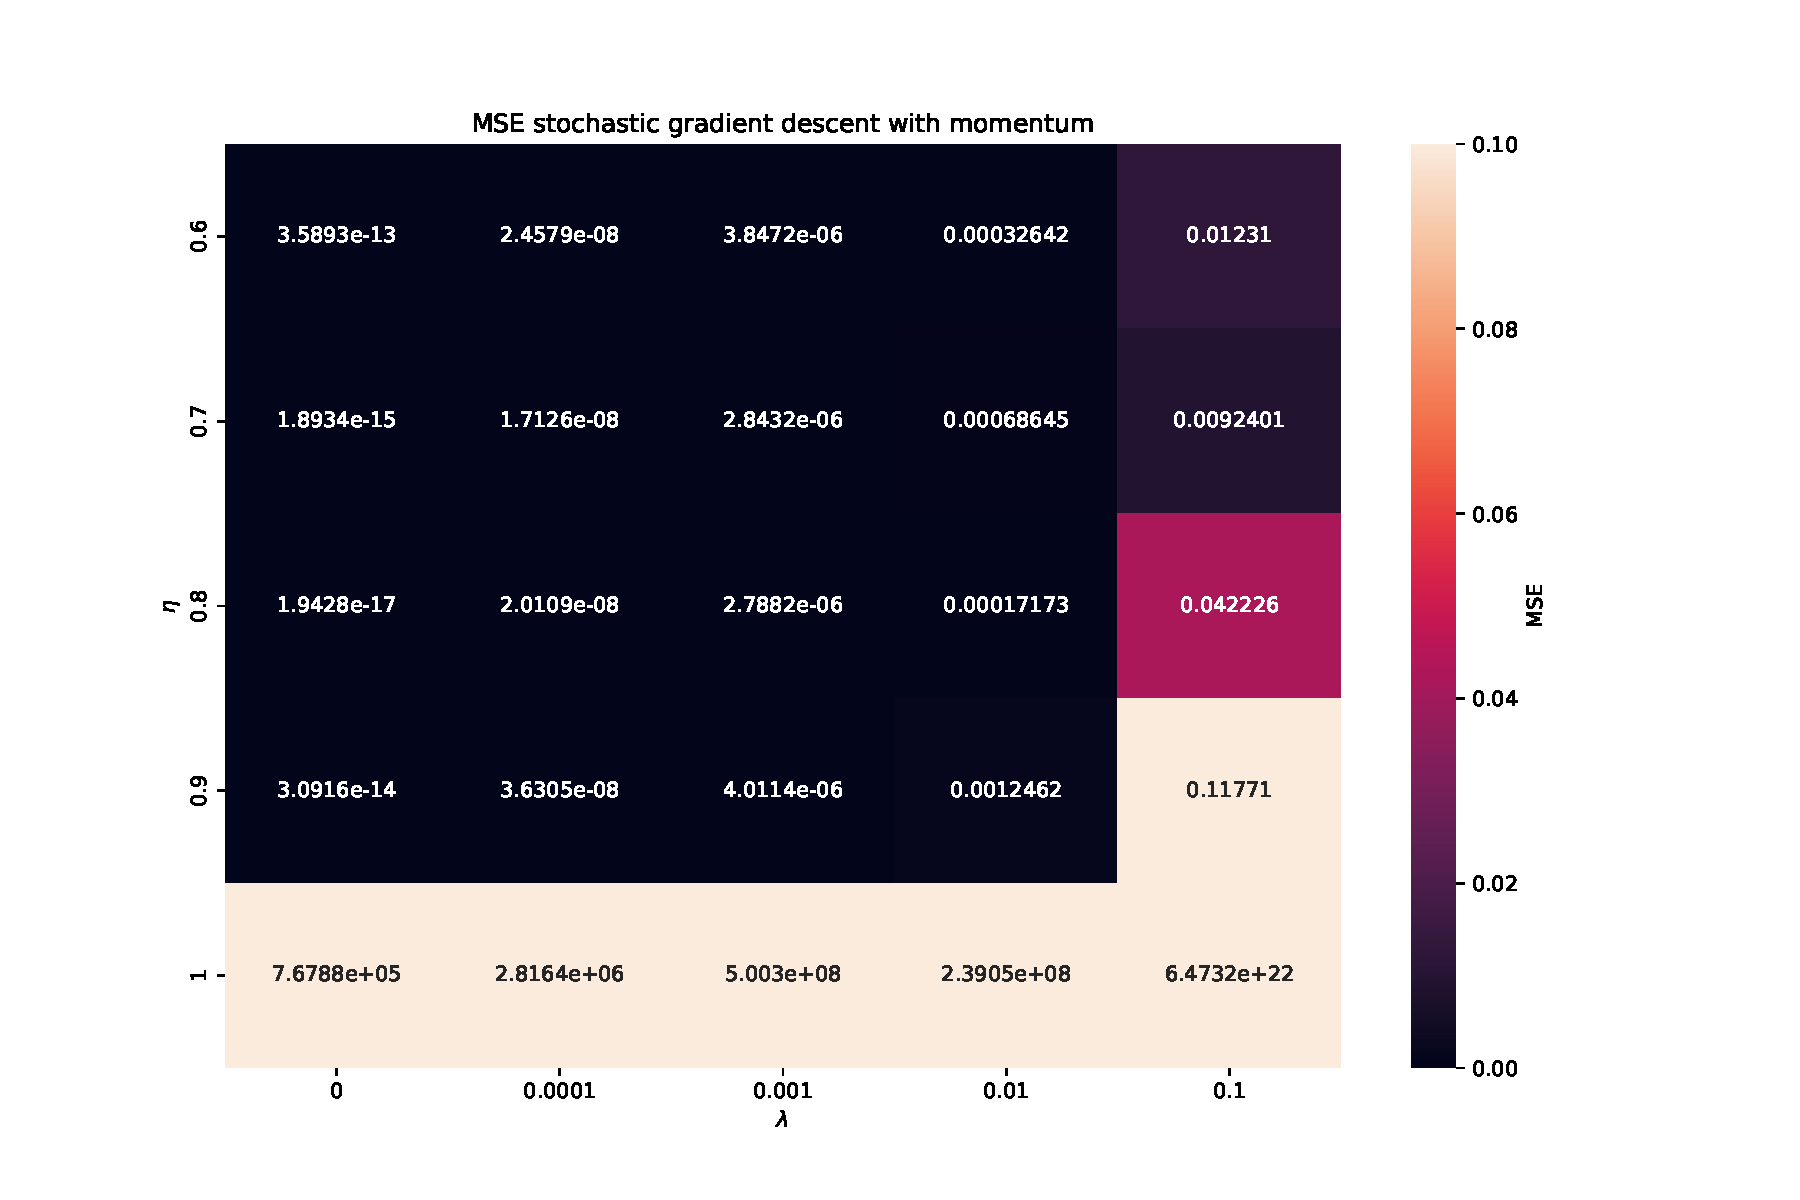
\includegraphics[width=0.8\textwidth]{Figures/PartA/sgdm_MSE(eta,lmb)}
\caption{Stochastic gradient descent with momentum: test MSE as a function of \(\eta \) and \(\lambda \).
 The parameters utilized are shown in table \ref{tab:GD_parameters_run_1_2} under run 1.}
\label{fig:sgdm_MSE-eta-lmb-}
\end{figure}

Figure \ref{fig:gd_MSE-eta-lmb-}-\ref{fig:sgdm_MSE-eta-lmb-} shows MSE scores of the test data for 
plain and stochastic gradient descent with and without momentum as a function of
different learning rates \(\eta \) and L2-regularzation parameters \(\lambda \). Both plain and 
stochastic gradient descent has the same amount of total iterations as there are $25$ sgd epochs 
and $n\_data/mini\_batch\_size=80/20=4$ minibatches giving a total amount of $25 \cdot 4 = 100$ 
iterations for stochastic gradient descent. We observe that we get a worse MSE score with larger 
learning rates up to a point where the score blows up shown for $\eta=1$. This makes sense as larger 
learning rates results in larger update to the parameters $\bf{\theta } $. Thus, too large learning reate 
will overshoot the minima of the cost function, while too small will cause slow convergence.  
We also observe the MSE to increase with increasing L2-regularzation parameter $\lambda $. This also 
makes sense as $\lambda $ counters overfitting at the cost of poorer training fit, but since we are 
optimizing the coefficients of a same order polynomial as the target, overfitting will not be a problem.
We are therefore better off without the L2-regularzation parameter. 

The momentum 
term is proportional to the previous variable change, such that the components of this vector term that overshoots will  
be in the opposite direction and thus causing less of a step wich is why we observe the MSE blowing up without momentum,
while not blowing up with momentum for $\eta =0.9$. Momentum also gives better scores as it allows for bigger steps
before the minima of the cost function is traversed. 

The performance of plain and stochastic gradient descent is similar, with plain being slightly better. As the 
cost functions are convex, there is no local minimas for plain gradient descent to get stuck on, such that the 
performance difference will come down to the randomly sampled minibatches in stochastic gradient descent. 



\begin{figure}[H]
\centering
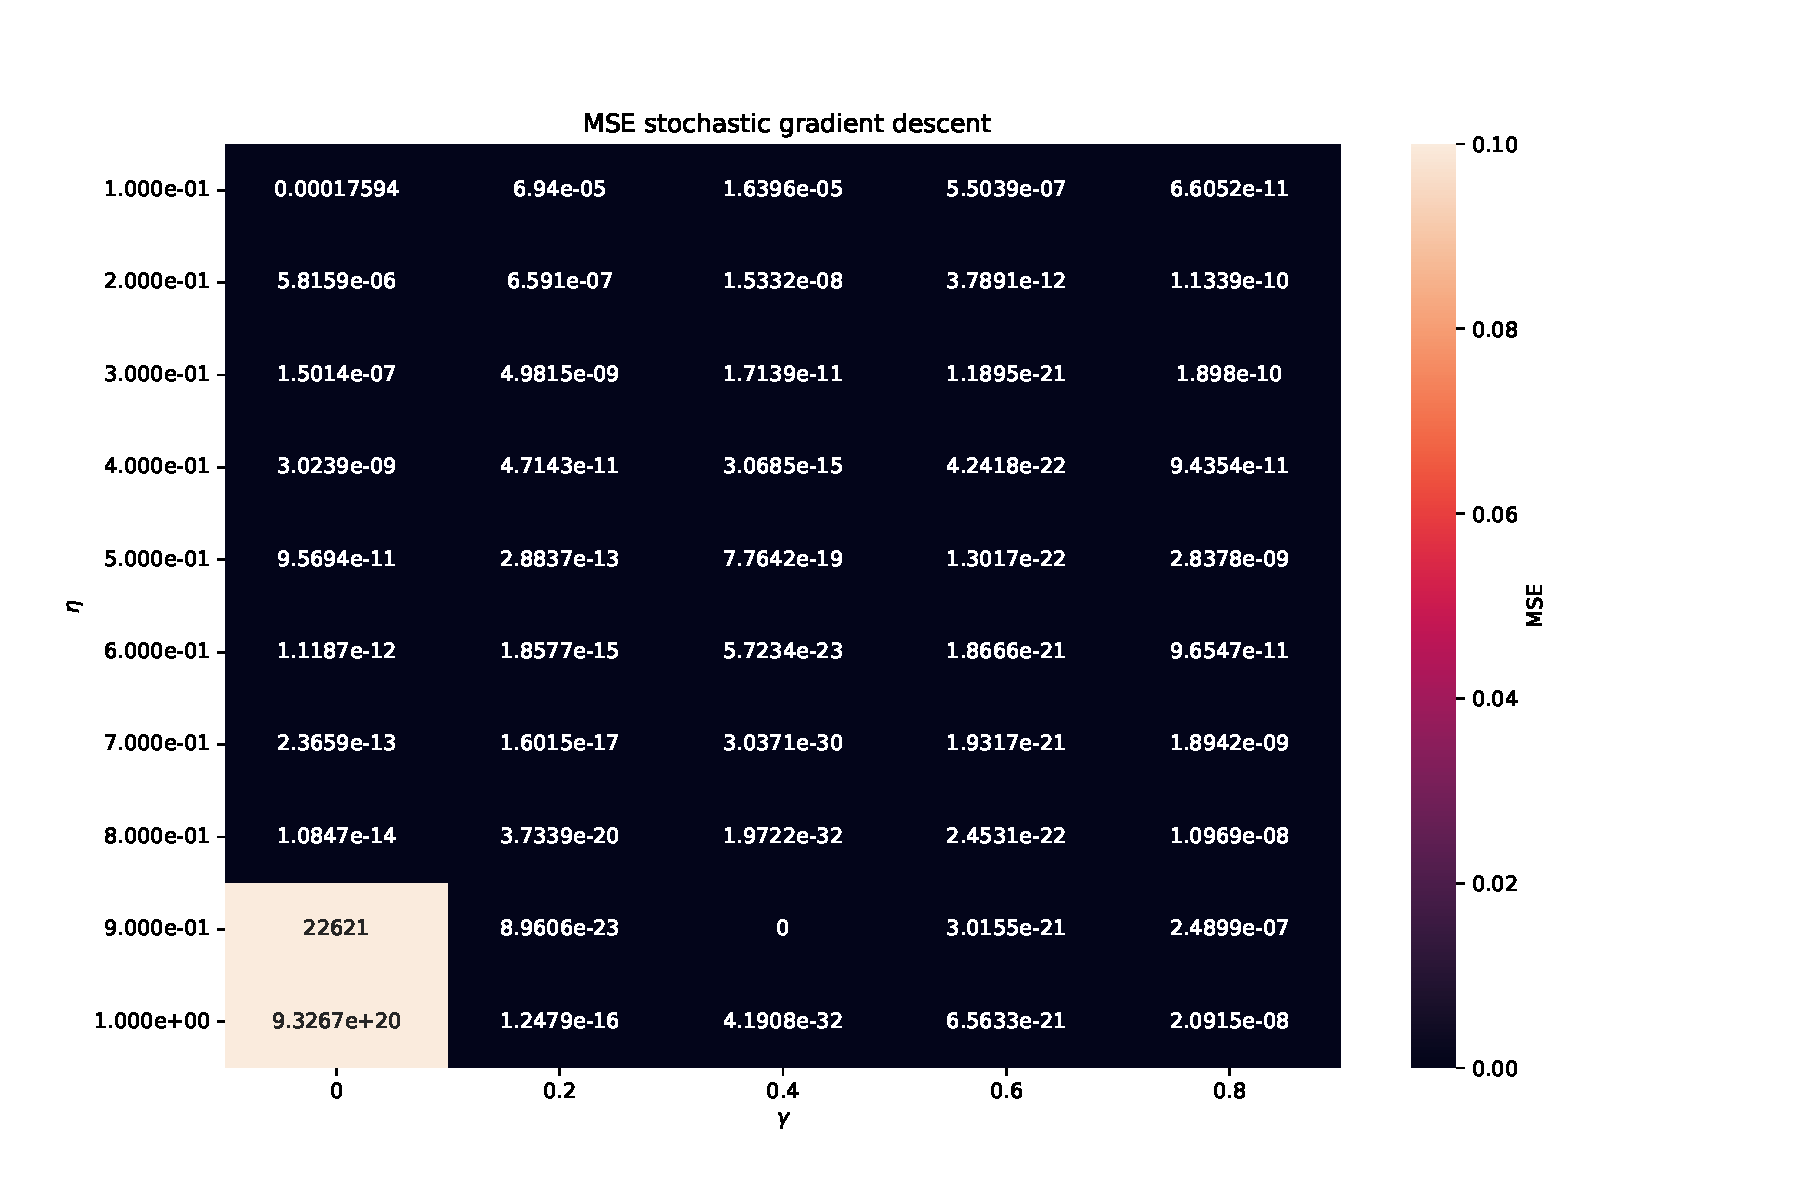
\includegraphics[width=0.8\textwidth]{Figures/PartA/_sgdm_MSE(eta,momentum)}
\caption{Stochastic gradient descent: MSE as a function of momentum parameter
    $\gamma$  and learning rate \(\eta \). The parameters utilized are shown in table \ref{tab:GD_parameters_run_1_2} under run 2	 }
\label{fig:_sgdm_MSE-eta-momentum-}
\end{figure}

\begin{figure}[H]
\centering
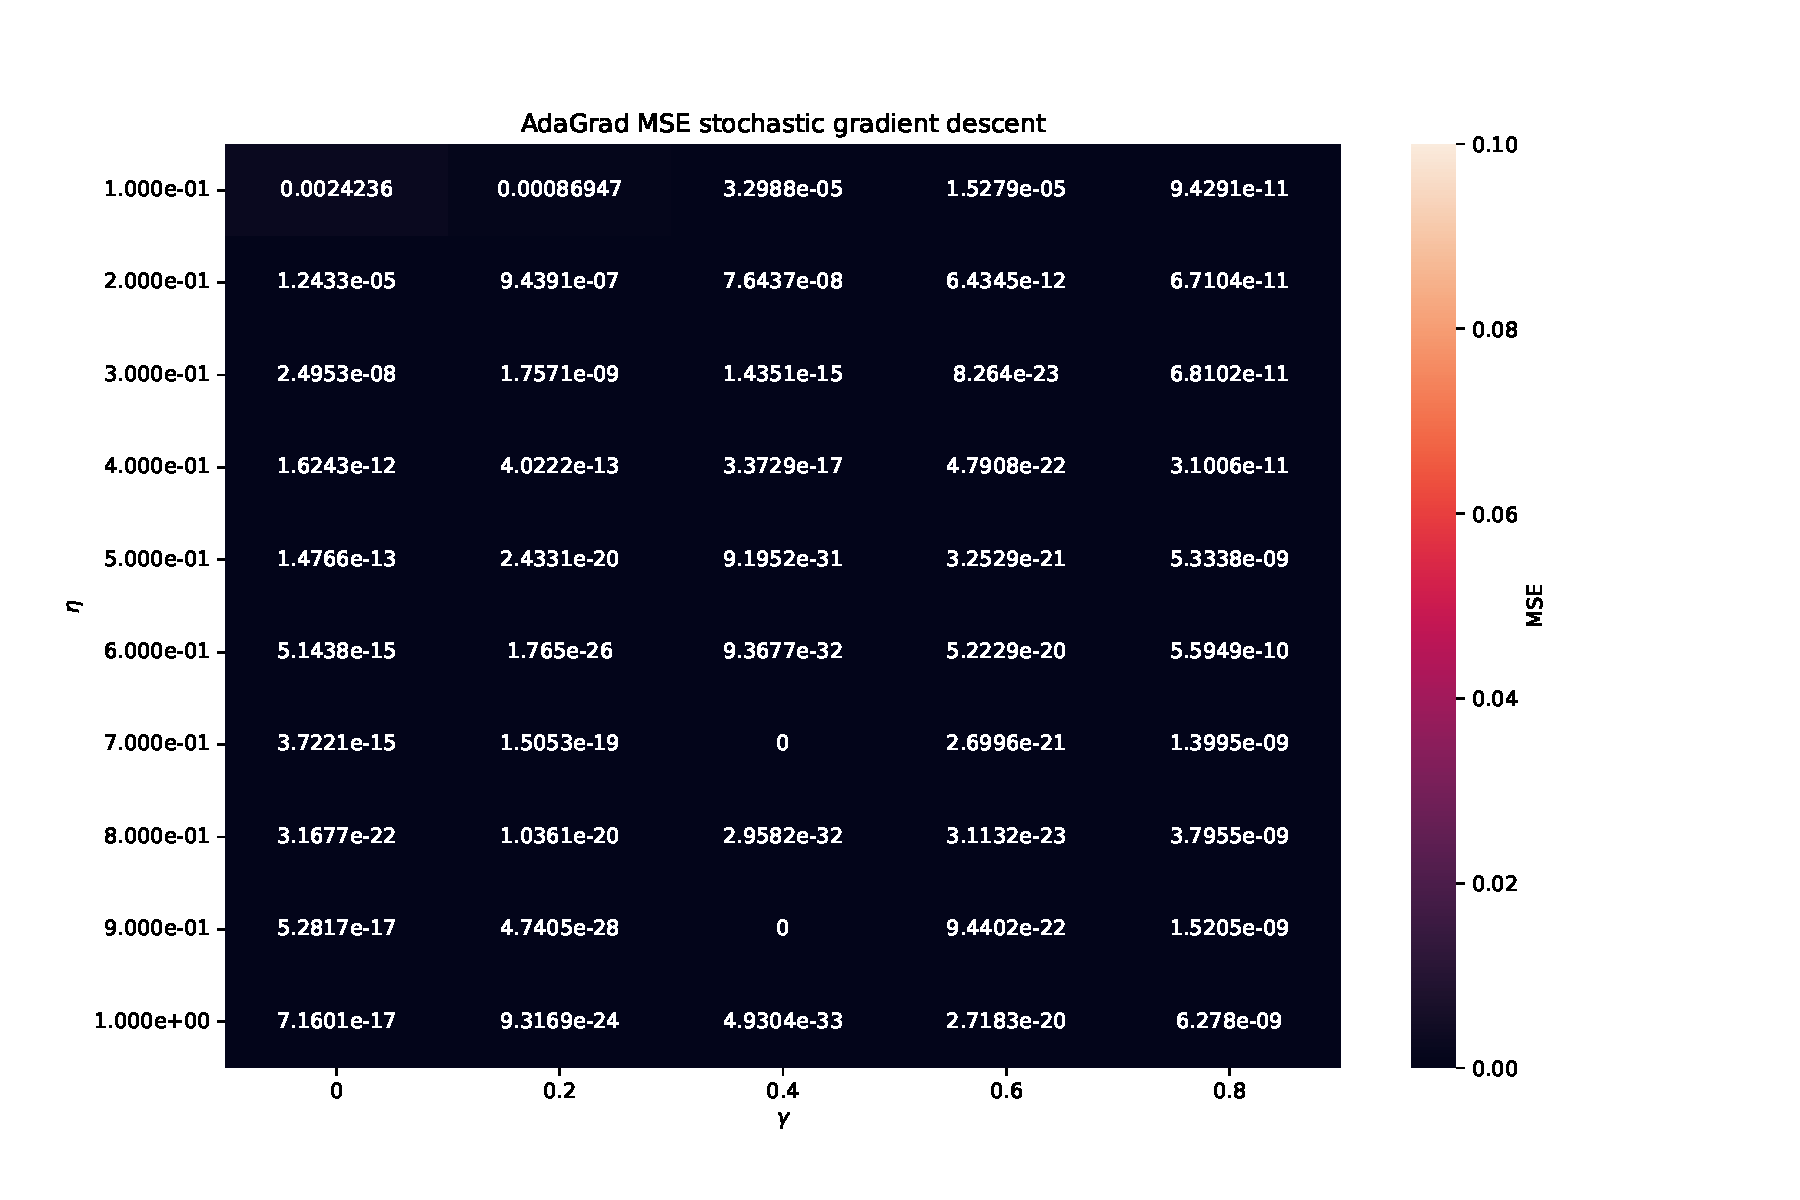
\includegraphics[width=0.8\textwidth]{Figures/PartA/AdaGrad_sgdm_MSE(eta,momentum)}
\caption{Stochastic gradient descent, with momentum and tuning method AdaGrad:
    MSE as a function of momentum parameter $\gamma$ and learning rate \(\eta \). The parameters utilized are shown in table \ref{tab:GD_parameters_run_1_2} under run 2	 }
\label{fig:AdaGrad_sgdm_MSE-eta-momentum-}
\end{figure}

\begin{figure}[H]
\centering
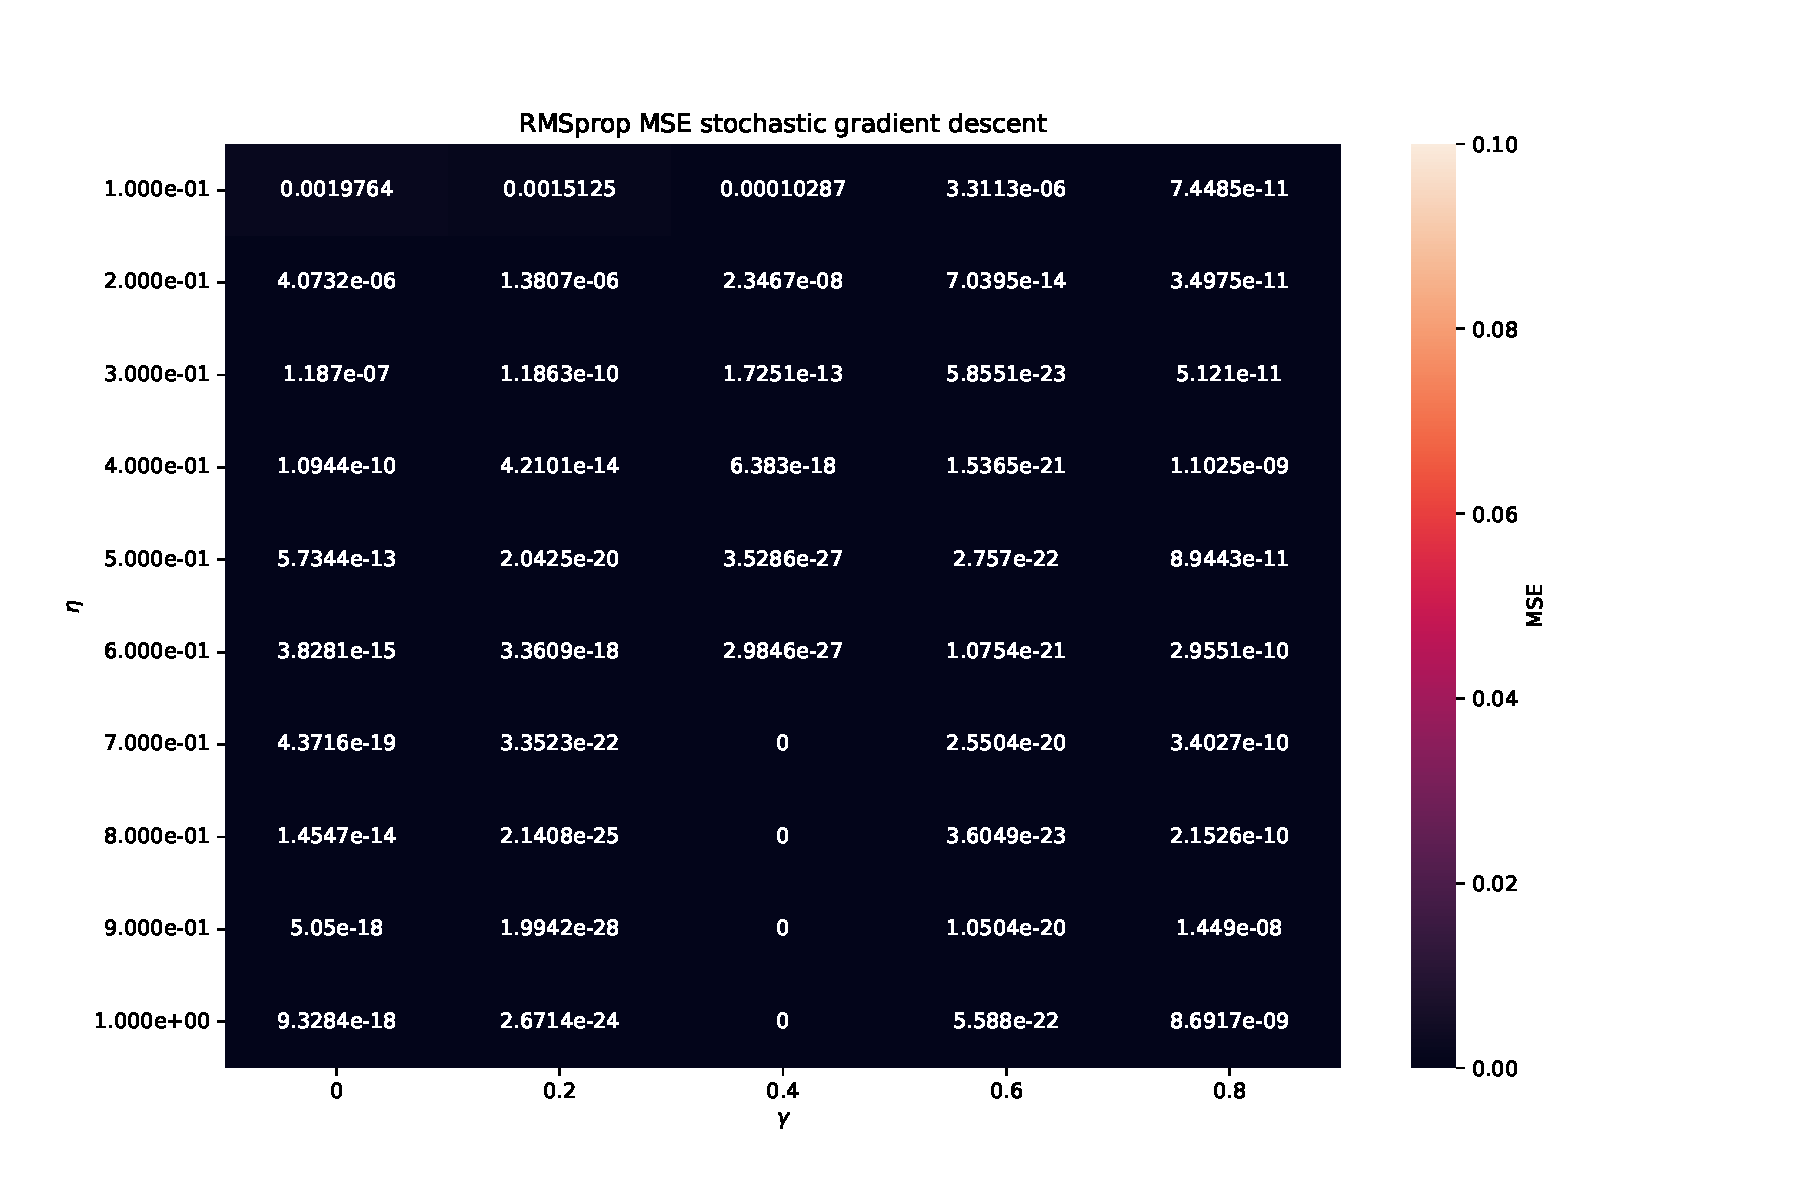
\includegraphics[width=0.8\textwidth]{Figures/PartA/RMSprop_sgdm_MSE(eta,momentum)}
\caption{Stochastic gradient descent, with momentum and tuning method
    RMSprop: MSE as a function of momentum parameter $\gamma$ and learning
    rate \(\eta \). The parameters utilized are shown in table \ref{tab:GD_parameters_run_1_2} under run 2	 }
\label{fig:RMSprop_sgdm_MSE-eta-momentum-}
\end{figure}

\begin{figure}[H]
\centering
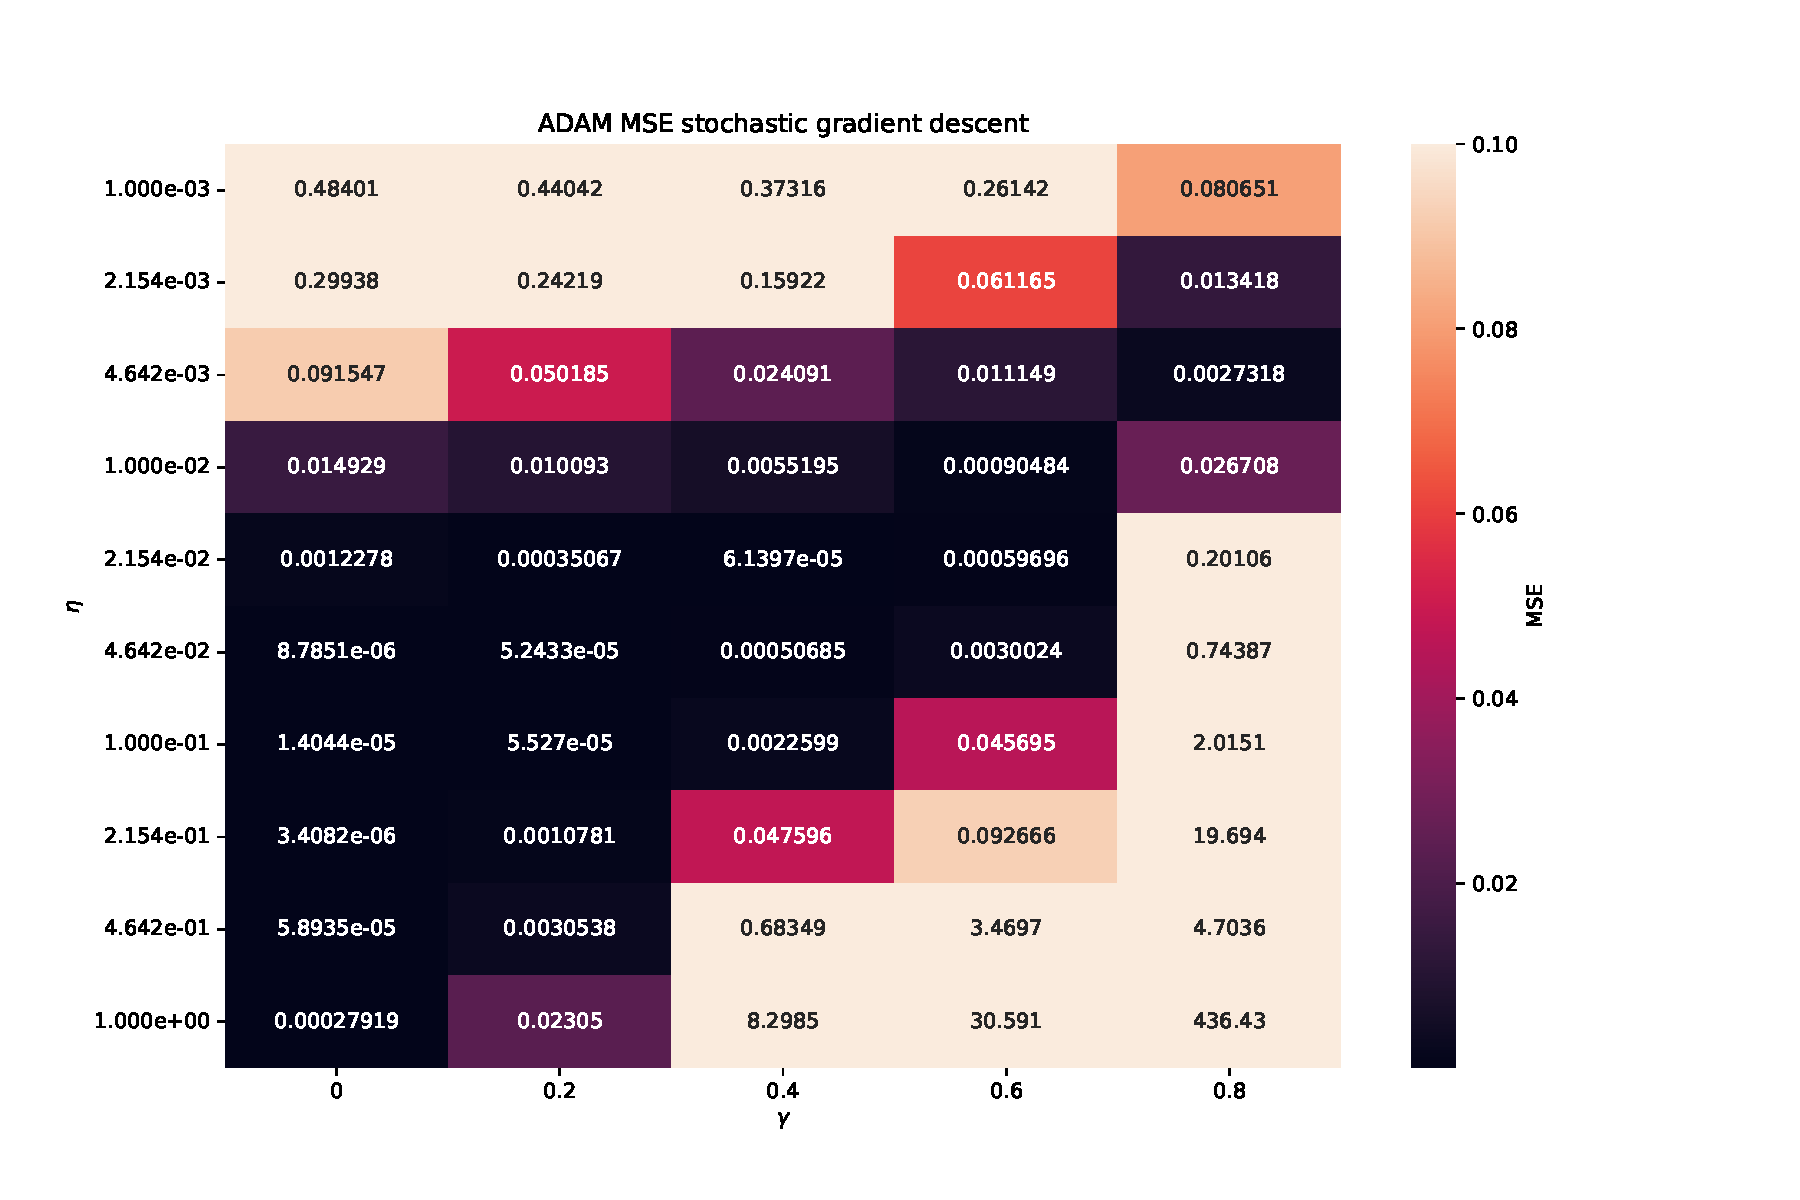
\includegraphics[width=0.8\textwidth]{Figures/PartA/ADAM_sgdm_MSE(eta,momentum)}
\caption{Stochastic gradient descent, with momentum and tuning method ADAM: MSE
    as a function of momentum parameter $\gamma$ and learning rate \(\eta \). The parameters utilized are shown in table \ref{tab:GD_parameters_run_3_4} under run 3	 }
\label{fig:ADAM_sgdm_MSE-eta-momentum-}
\end{figure}

Figure \ref{fig:_sgdm_MSE-eta-momentum-}-\ref{fig:ADAM_sgdm_MSE-eta-momentum-}, shows the MSE from stochastic gradient descent for different
learning rates $\eta $ and momentum parameters $\gamma $ for no tuning method, AdaGrad, RMSprop and ADAM. We observe that ADAM does not benefit 
from momentum, while AdaGrad, RMSprop, and plain stochastic gradient descent shows best results for momentum parameter $\gamma =0.4$ with appropriate 
learning rates $\eta $.  


\begin{figure}[H]
\centering
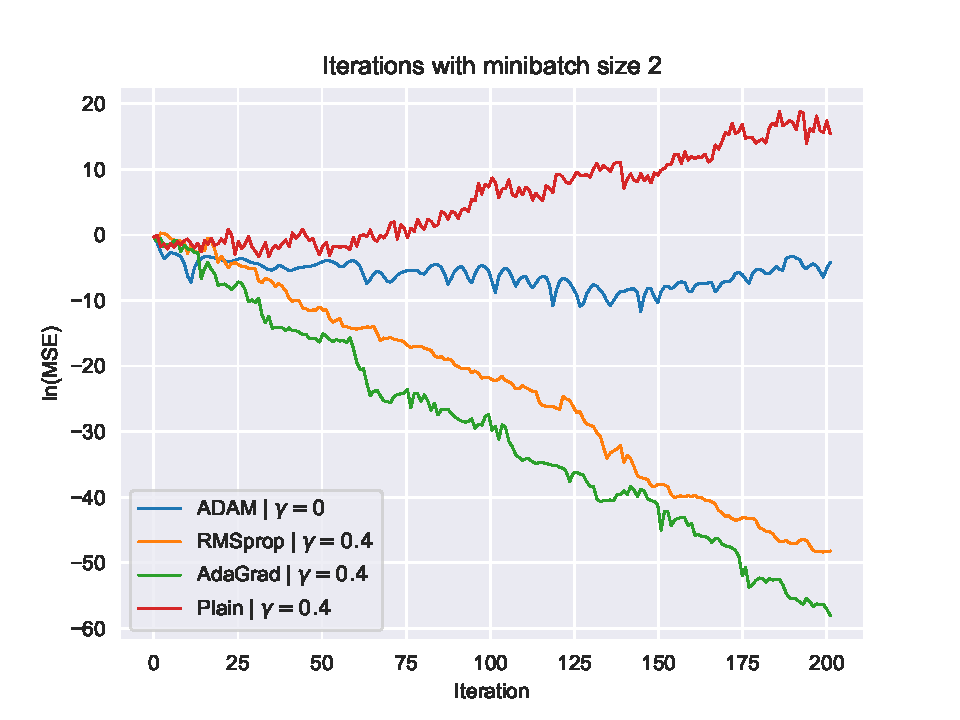
\includegraphics[width=0.8\textwidth]{Figures/PartA/minibatch_2_MSE(iter).pdf}
\caption{Stochastic gradient descent using plain, AdaGrad, RMSprop and ADAM as tuning methods: ln(MSE) as a function of iterations with minibatch size 2.
The parameters utilized are shown in table \ref{tab:GD_parameters_run_3_4} under run 4.}
\label{fig:minibatch_2_MSE-iter}
\end{figure}

\begin{figure}[H]
\centering
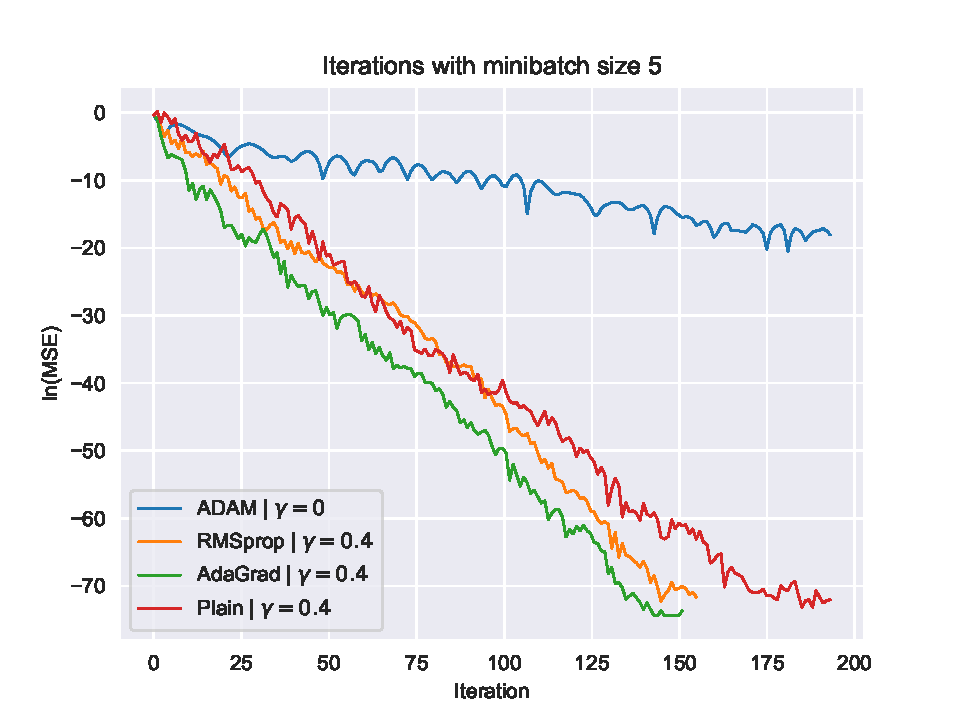
\includegraphics[width=0.8\textwidth]{Figures/PartA/minibatch_5_MSE(iter).pdf}
\caption{Stochastic gradient descent using plain, AdaGrad, RMSprop and ADAM as tuning methods: ln(MSE) as a function of iterations with minibatch size 5.
 The parameters utilized are shown in table \ref{tab:GD_parameters_run_3_4} under run 4.}
\label{fig:minibatch_5_MSE-iter}
\end{figure}

\begin{figure}[H]
\centering
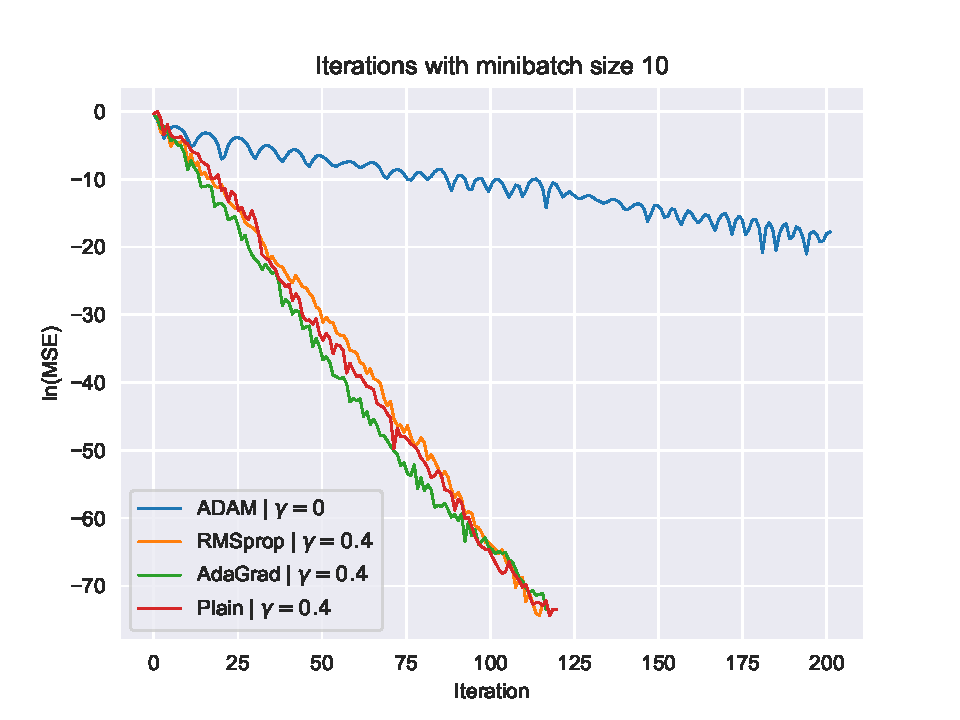
\includegraphics[width=0.8\textwidth]{Figures/PartA/minibatch_10_MSE(iter).pdf}
\caption{Stochastic gradient descent using plain, AdaGrad, RMSprop and ADAM as tuning methods: ln(MSE) as a function of iterations with minibatch size 10.
 The parameters utilized are shown in table \ref{tab:GD_parameters_run_3_4} under run 4.}
\label{fig:minibatch_10_MSE-iter}
\end{figure}

\begin{figure}[H]
\centering
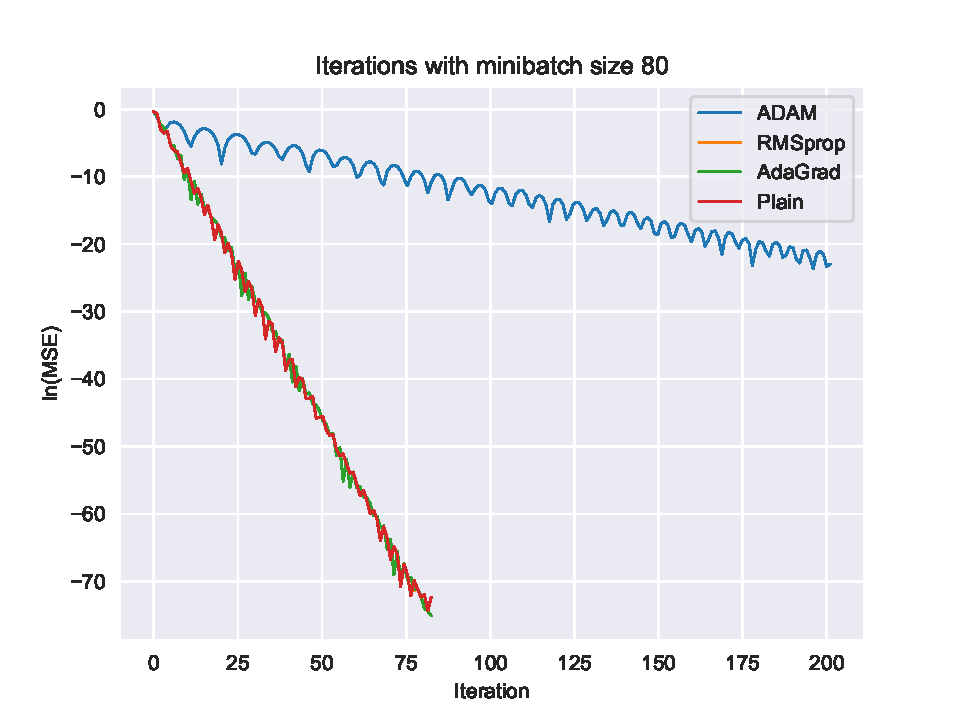
\includegraphics[width=0.8\textwidth]{Figures/PartA/minibatch_80_MSE(iter).pdf}
\caption{Stochastic gradient descent using plain, AdaGrad, RMSprop and ADAM as tuning methods: ln(MSE) as a function of iterations with minibatch size 80.
 The parameters utilized are shown in table \ref{tab:GD_parameters_run_3_4} under run 4.}
\label{fig:minibatch_80_MSE-iter}
\end{figure}

Figure \ref{fig:minibatch_2_MSE-iter}-\ref{fig:minibatch_80_MSE-iter} shows the natural logarithm of MSE as a function of iterations
for minibatch size 2, 5, 10 and 80 respectively. Each figure shows stochastic gradient descent with momentum parameter $\gamma $ for no tuning method (plain),
tuning method AdaGrad, RMSprop and ADAM utilized to fit the polynomial in equation \ref{eq:polynomial_A}. As the training data 
size is 80, minibatch size 80 corresponds to non-stochastic gradient descent. The reason the plots dissapear in the vicinity of $y=-70$ 
is that the MSE traverses the lowest positive number possible in python such that they are set to zero wich is undefined in the logarithm function. 
We observe faster convergence with larger minibatch sizes for all the methods. No tuning method, AdaGrad and RMSprop have similar performance for minibatch 
sizes 80 and 10. For smaller sizes, we observe that AdaGrad performs best closely followed by RMSprop, while Plain starts deviating and is its MSE is 
exploding for minibatch size 2. ADAM performs worst (except compared to the exploding Plain) and is converging quite a lot slower, allthough the difference 
seems to lessen with smaller minibatch size. Smaller minibatch size introduces the probability of more variance in the gradient which suggests ADAM might be more 
applicable to more complex cost functions.    

%%%% TODO: Write about this, but first find out why adam is so wierd
%%%%%%%%%%%%%%%%%%%%
\begin{comment}
In figure \ref{fig:minibatch_2_MSE-iter-pdf} -
\ref{fig:minibatch_80_MSE-iter-pdf} we can see the MSE as a function of
iterations for 2, 5, 10 and 80 minibatch sizes. And we note that the bigger the
minibatch, the smaller the MSE gets by each iteration. This makes sense as you
include more and more of the training set and would therefore expect the MSE to
get smaller. 
\end{comment}
%%%%%%
%%%%%%%

\begin{figure}[H]
\centering
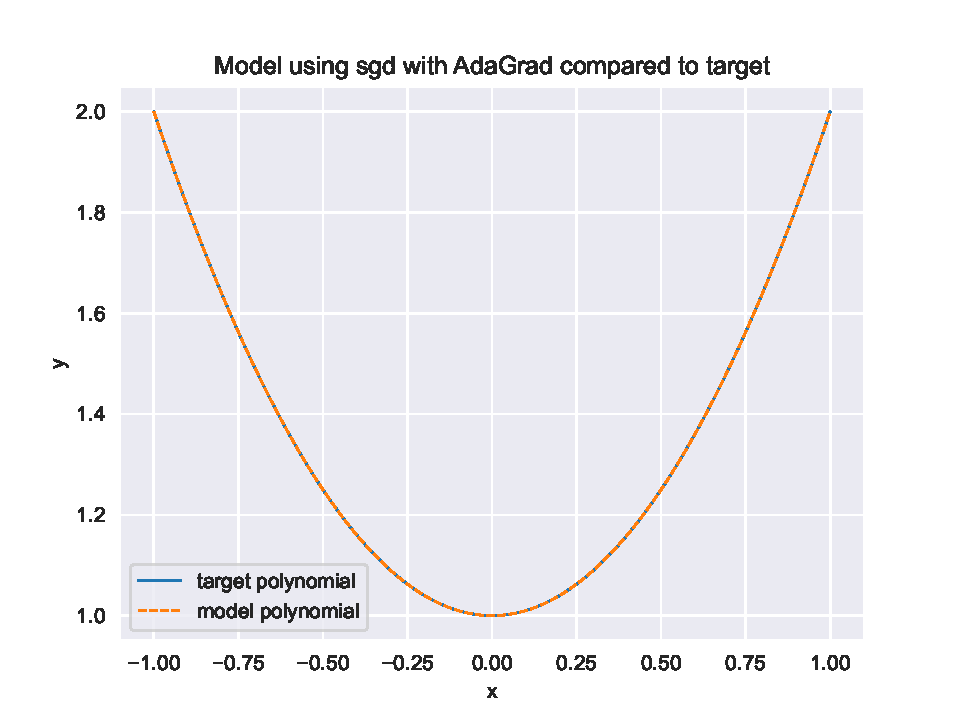
\includegraphics[width=0.8\textwidth]{Figures/PartA/sgd_polynomial_fit}
\caption{Resulting polynomial after stochastic gradient descent with optimizer AdaGrad compared to the target function.
 The parameters utilized are shown in table \ref{tab:GD_parameters_run_5}}
\label{fig:sgd_polynomial_fit}
\end{figure}

Figure \ref{fig:sgd_polynomial_fit} shows the resulting polynomial from stochastic gradient descent with tuning method AdaGrad compared 
to the target polynomial. As expected from the MSE analysis, the prediction is perfect at eye level. A perfect fit could also easily be achived 
with for example ordinary least squares, allthough this is computationally heavy for huge datasets where the option of using minibatches in 
stochastic gradient descent would be beneficial. 

\subsection{Neural Network Regression}

\begin{figure}[H]
    \centering
    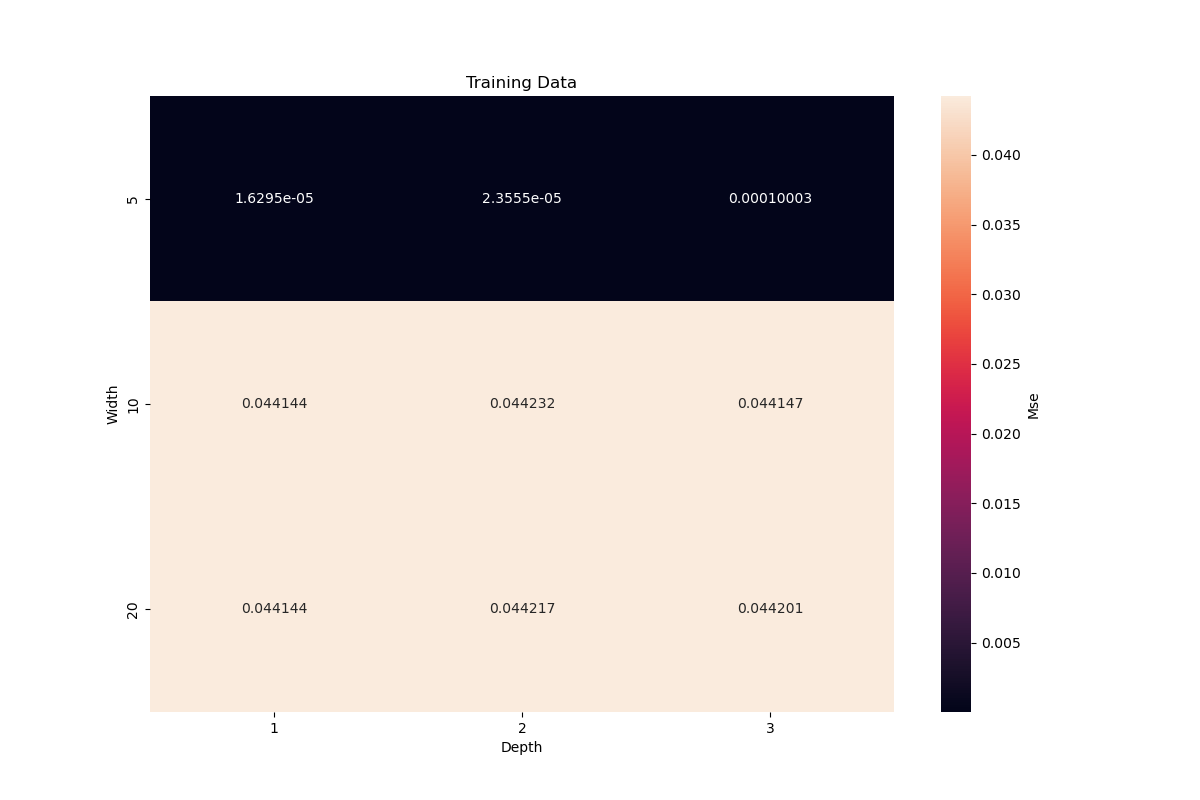
\includegraphics[width=0.8\textwidth]{Figures/PartB/heatmap_train_polydata_width_vs_depth.png}
    \caption{MSE score predicted on the polynomial training data with respect
    different number of hidden nodes (Width) and layers (Depth). Parameters
used is listed in table \ref{tab:NN_polynomial_parameters3} under Run 6.}  
    \label{fig:polydata_train_width_vs_depth} 

\end{figure}

\begin{figure}[H]
    \centering
    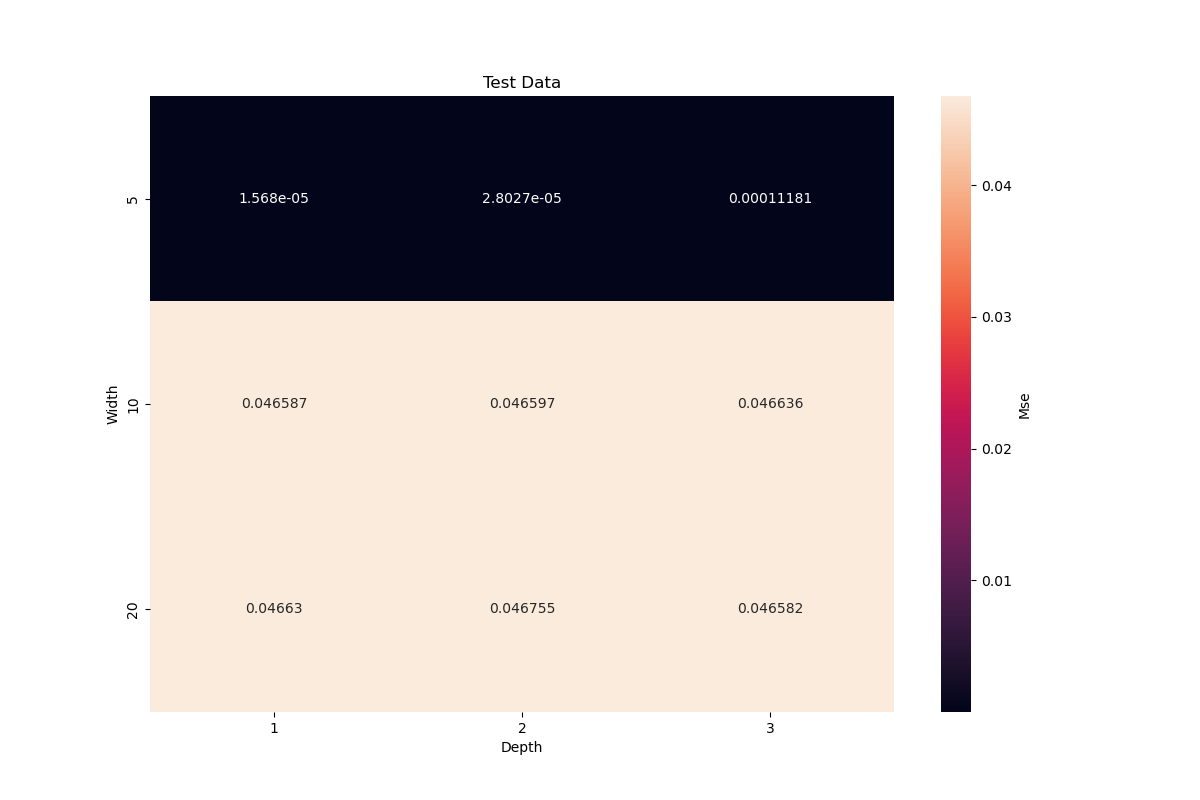
\includegraphics[width=0.8\textwidth]{Figures/PartB/heatmap_test_polydata_width_vs_depth.png}
    \caption{MSE score predicted on the polynomial test data with respect
    different number of hidden nodes (Width) and layers (Depth). Parameters
used is listed in table \ref{tab:NN_polynomial_parameters3} under Run 6.}  
    \label{fig:polydata_test_width_vs_depth} 
\end{figure}


Figure \ref{fig:polydata_train_width_vs_depth} and figure \ref{fig:polydata_test_width_vs_depth} shows 
respectively training and test MSE for different numbers of hidden layers, and different numbers of 
nodes in the hidden layer(s). The best MSE was obtained 
with 1 hidden layer consisting of 5 nodes. With width 10 and 20, the network gets stuck on training MSE around
$0.044$, such that less width should be explored when searching for optimal structure.  

\begin{figure}[htpb]
\begin{subfigure}{.5\textwidth}
  \centering
  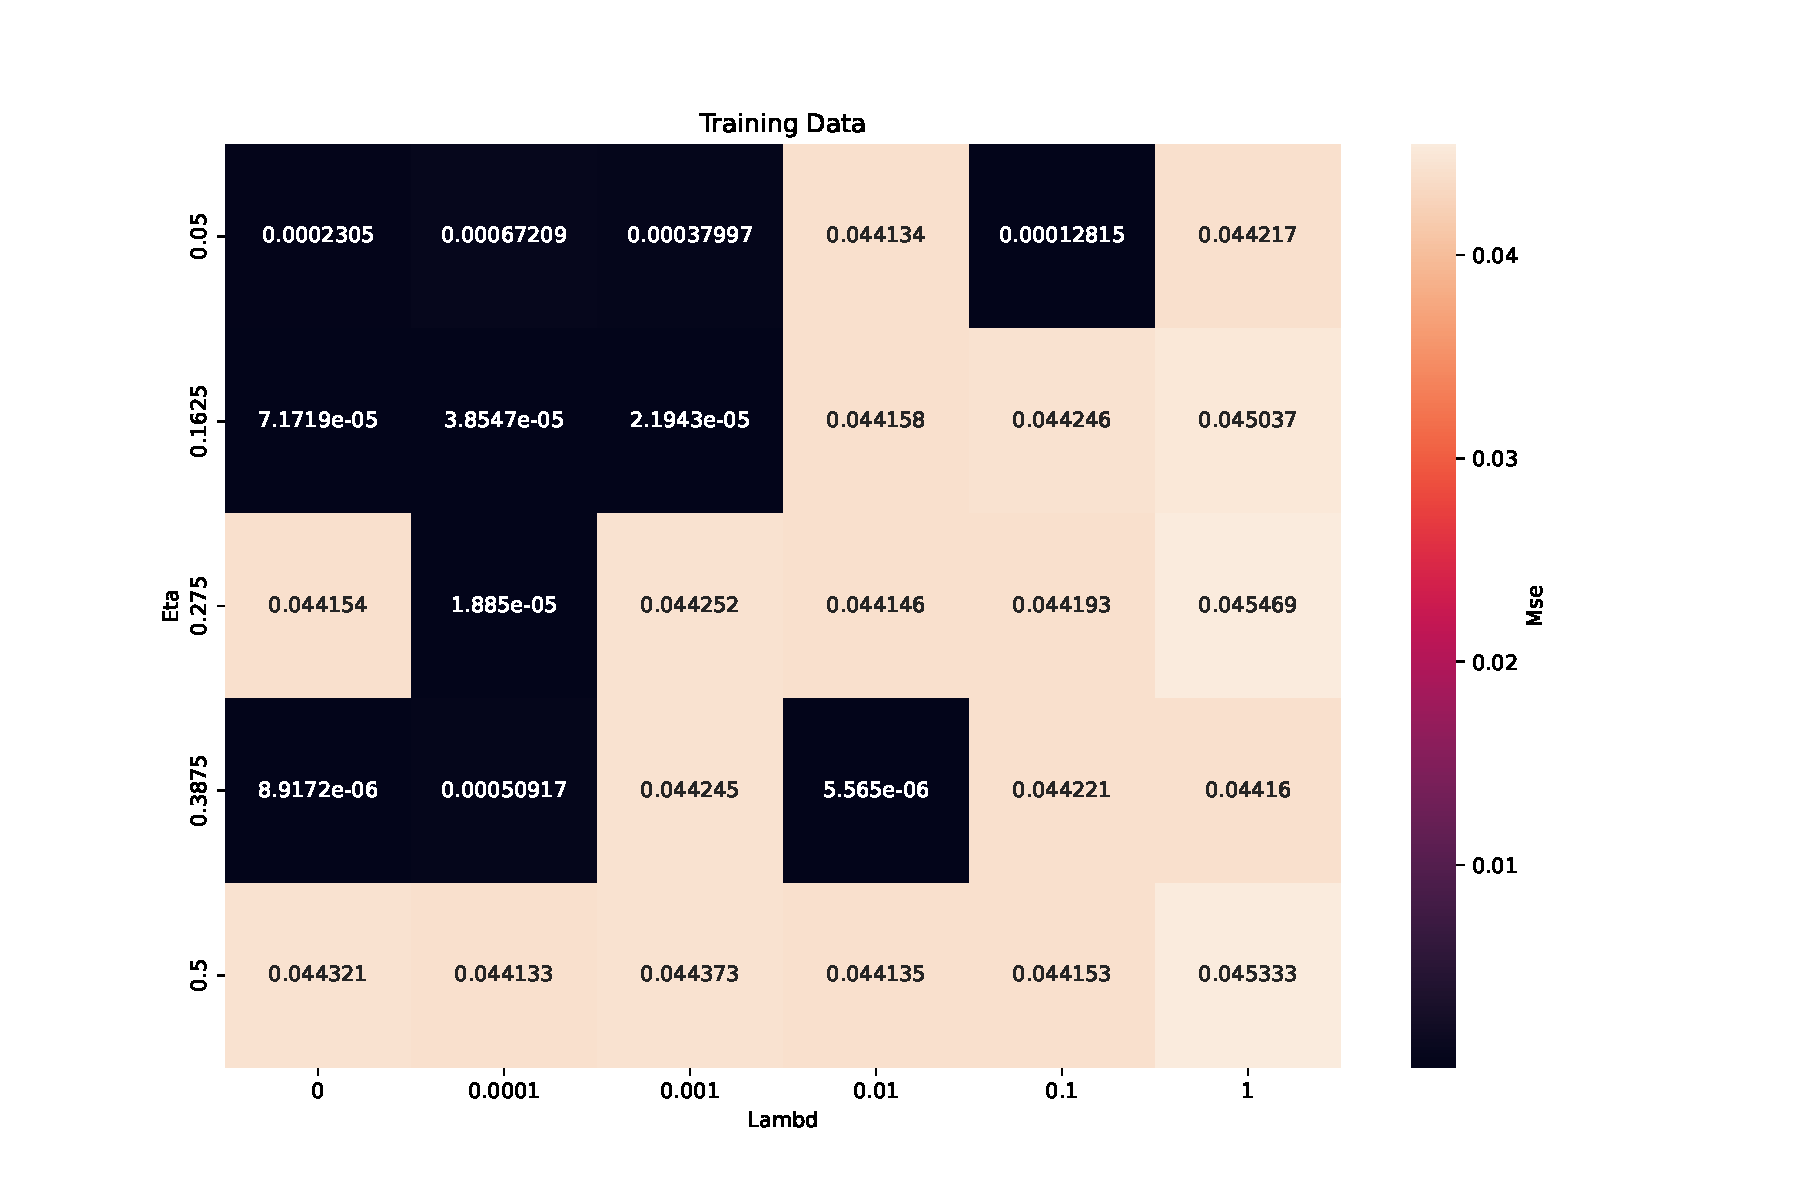
\includegraphics[width=1.1\linewidth]{Figures/PartB/train_sigmoid_MSE(eta,lmb)}
  \caption{Train MSE}
  \label{fig:train_sigmoid_MSE-eta-lmb-}
\end{subfigure}%
\begin{subfigure}{.5\textwidth}
  \centering
  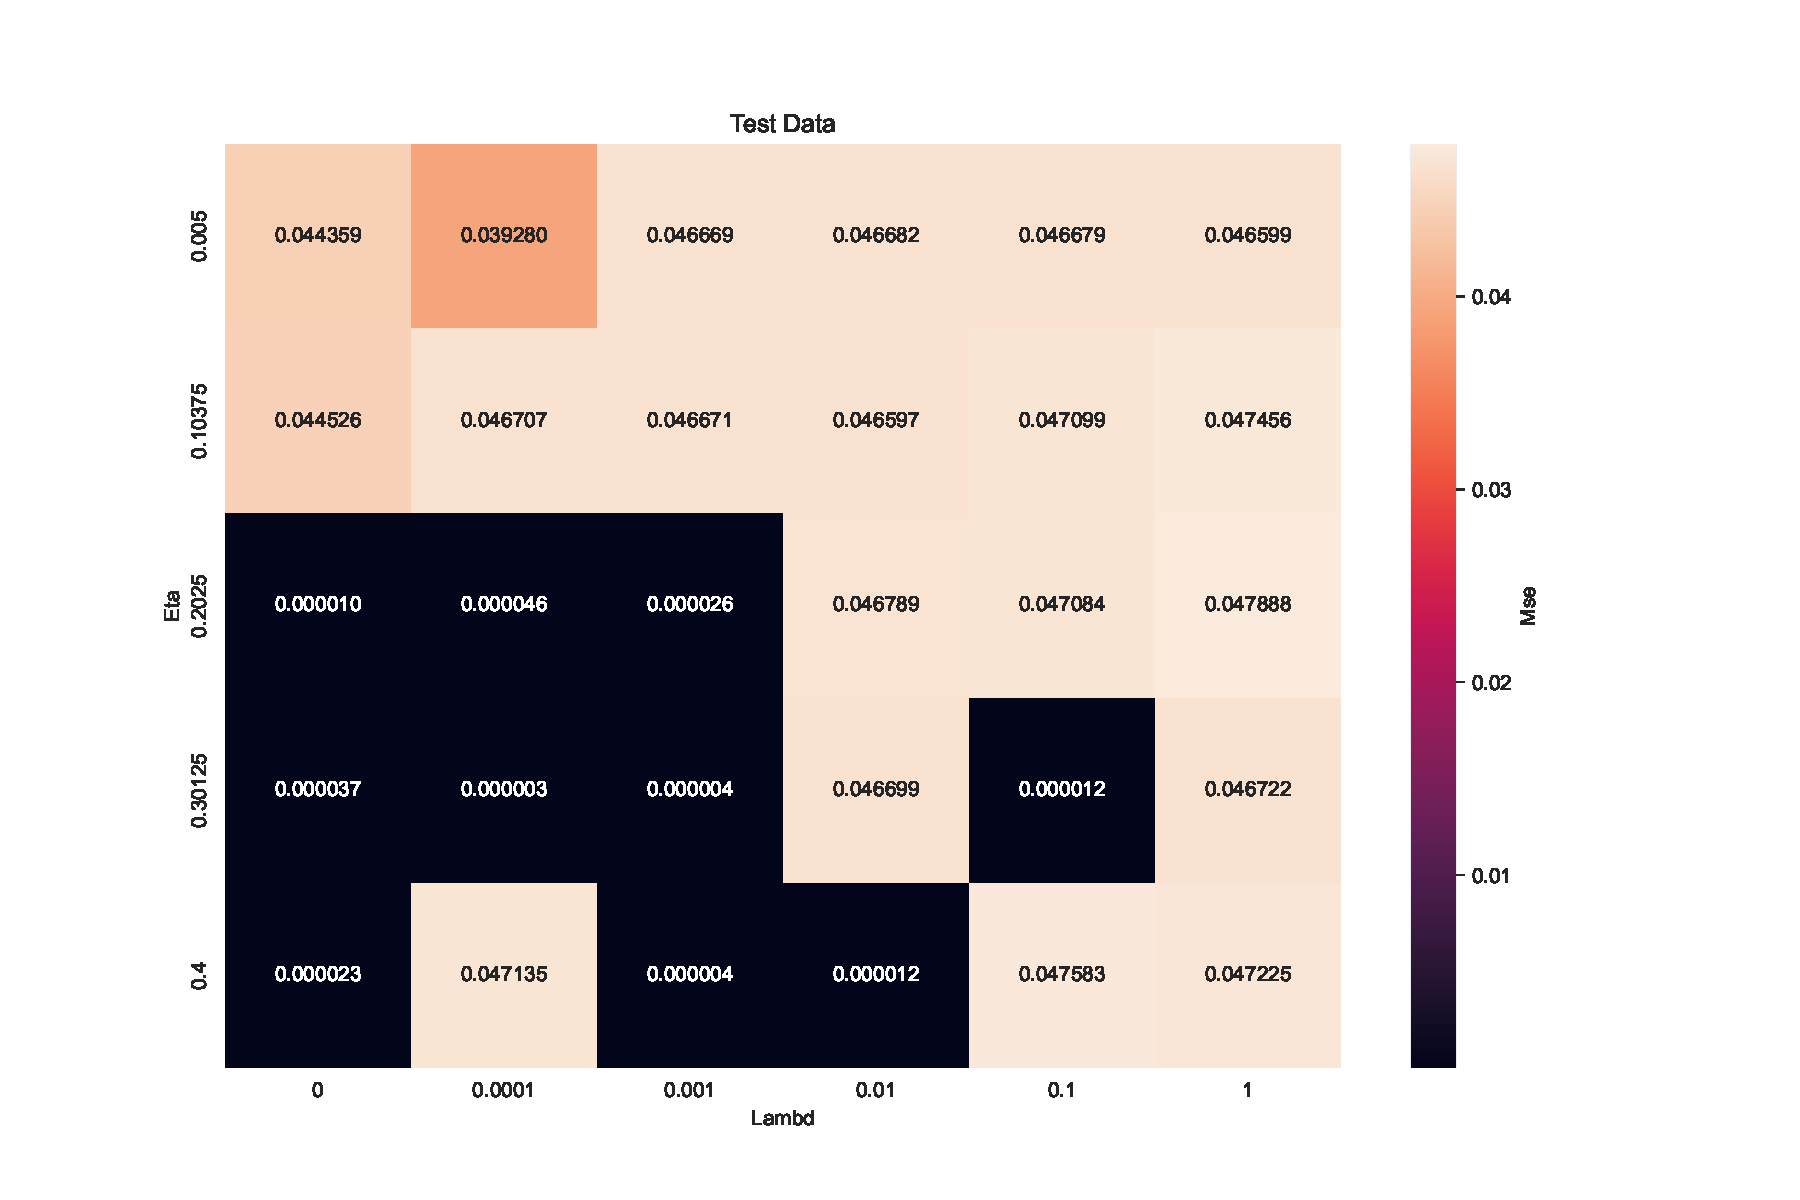
\includegraphics[width=1.1\linewidth]{Figures/PartB/test_sigmoid_MSE(eta,lmb)}
  \caption{Test MSE}
  \label{fig:test_sigmoid_MSE-eta-lmb-}
\end{subfigure}
\caption{Neural network with activation function Sigmoid: MSE as a function of \(\eta \) and \(\lambda \).
The parameters utilized are shown in table \ref{tab:NN_polynomial_parameters1} under run 1.}
\label{fig:Sigmoid_MSE}
\end{figure}

\begin{figure}[htpb]
\begin{subfigure}{.5\textwidth}
  \centering
  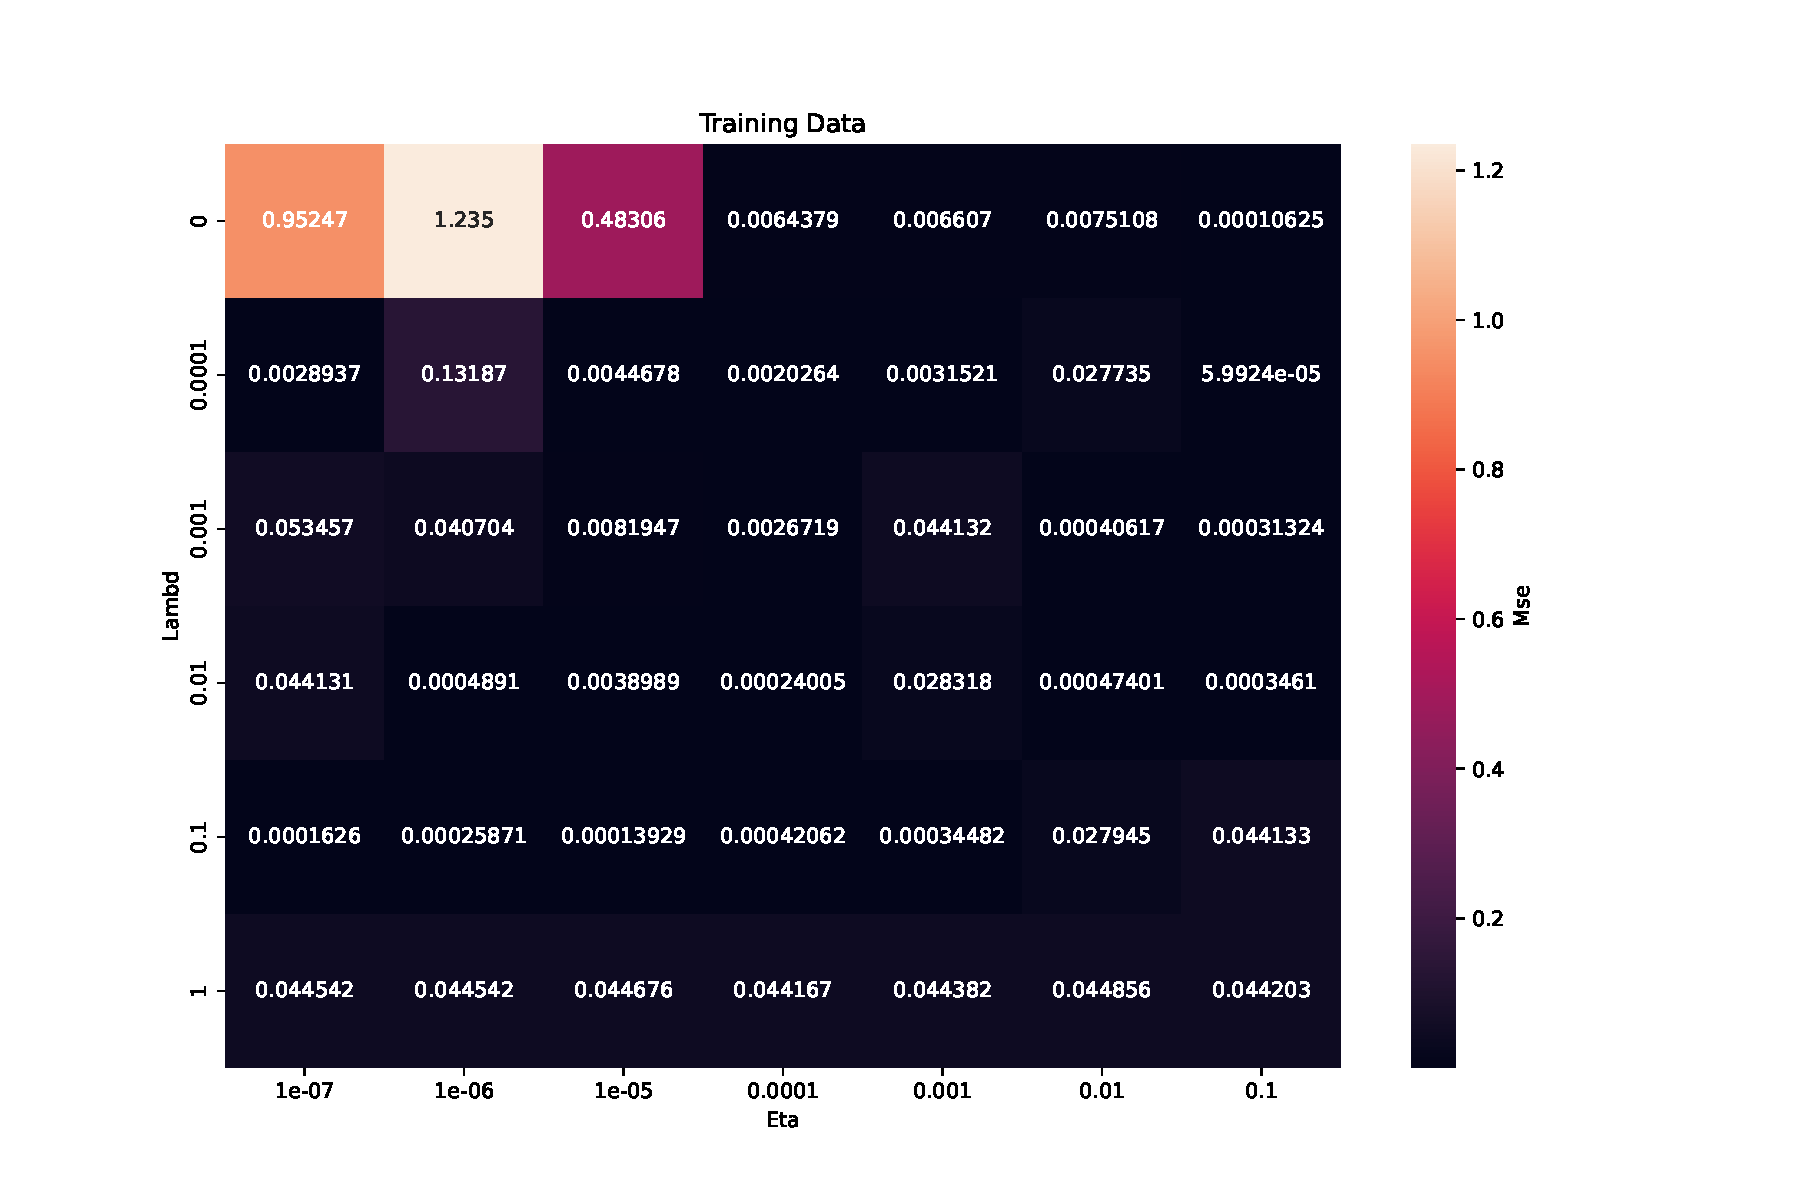
\includegraphics[width=1.1\linewidth]{Figures/PartB/train_relu_MSE(eta,lmb)}
  \caption{Train MSE}
  \label{fig:train_relu_MSE-eta-lmb-}
\end{subfigure}%
\begin{subfigure}{.5\textwidth}
  \centering
  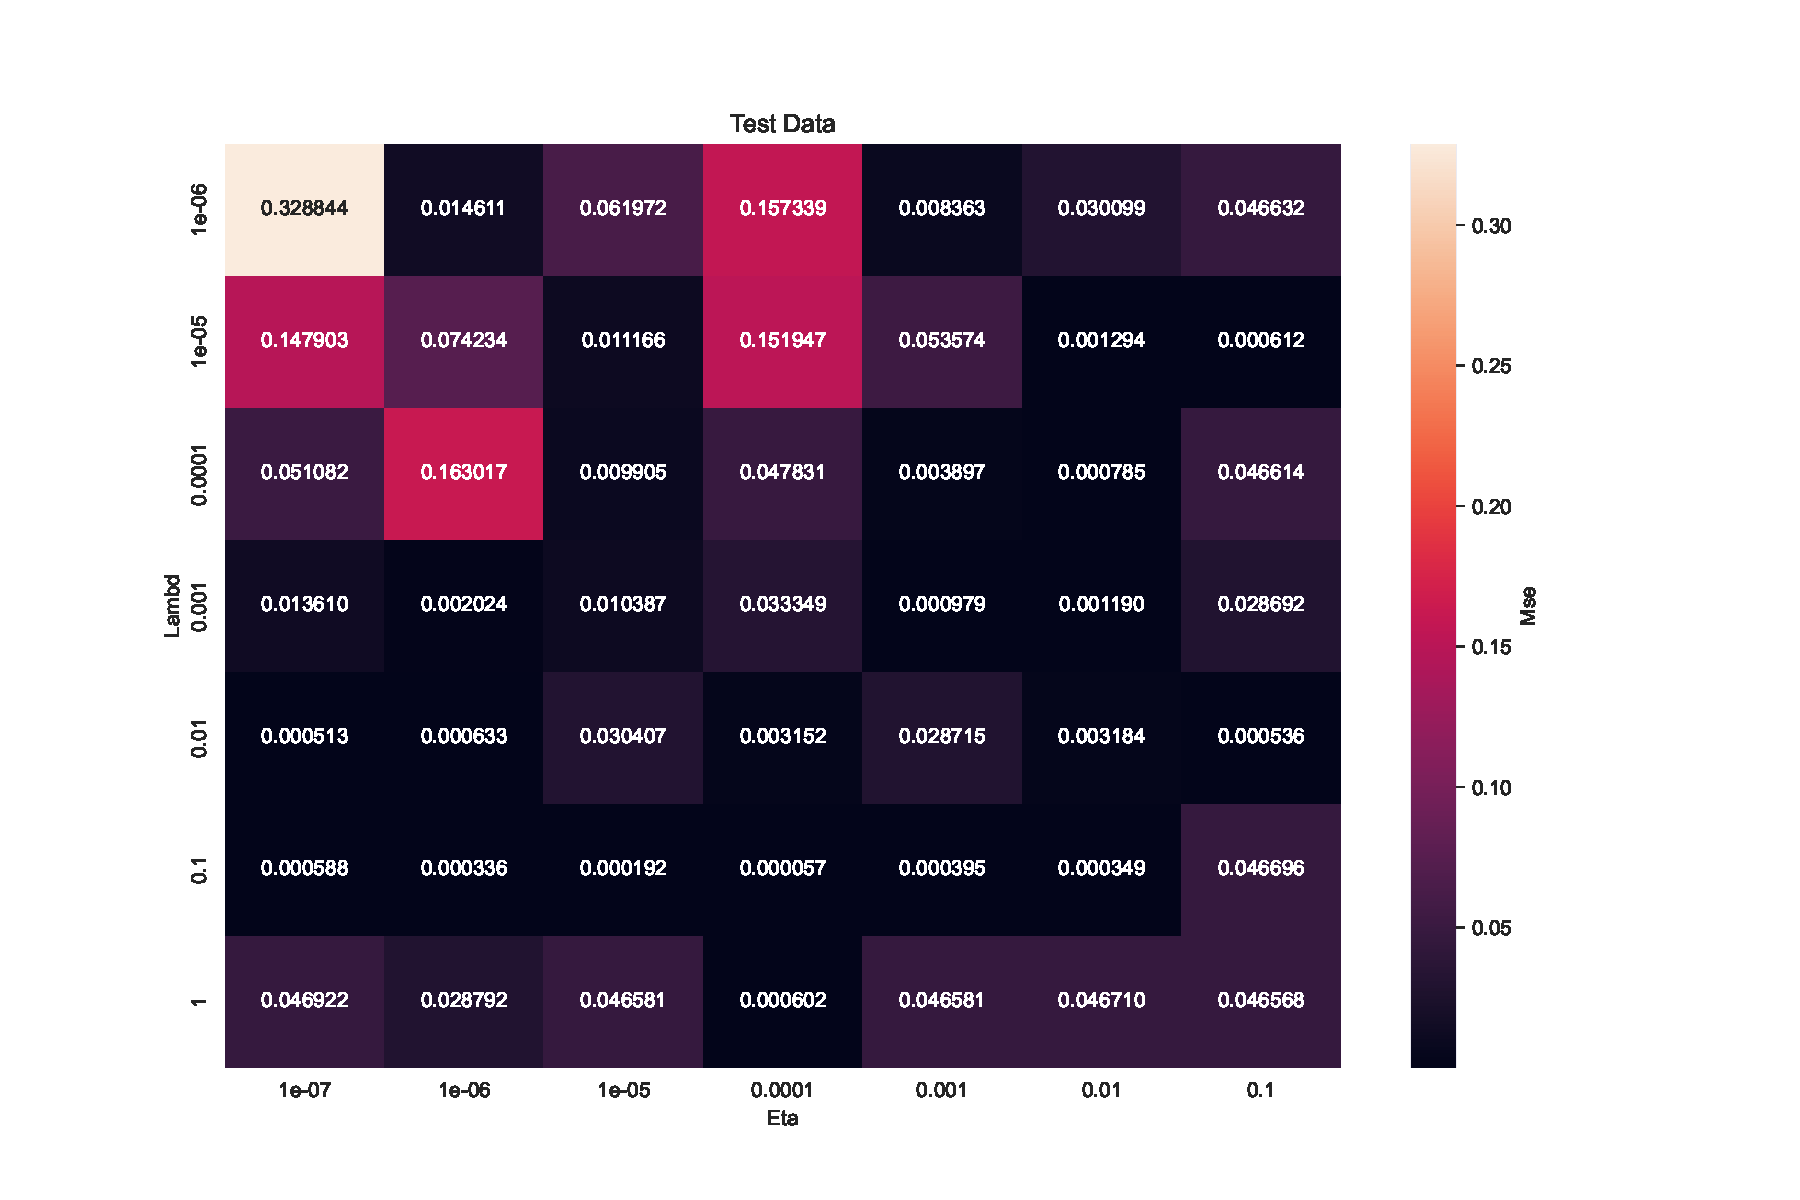
\includegraphics[width=1.1\linewidth]{Figures/PartB/test_relu_MSE(eta,lmb)}
  \caption{Test MSE}
  \label{fig:test_relu_MSE-eta-lmb-}
\end{subfigure}
\caption{Neural network with activation function relu: MSE as a function of \(\eta \) and \(\lambda \).
 The parameters utilized are shown in table \ref{tab:NN_polynomial_parameters1} under run 2.}
\label{fig:relu_MSE}
\end{figure}

\begin{figure}[htpb]
\begin{subfigure}{.5\textwidth}
  \centering
  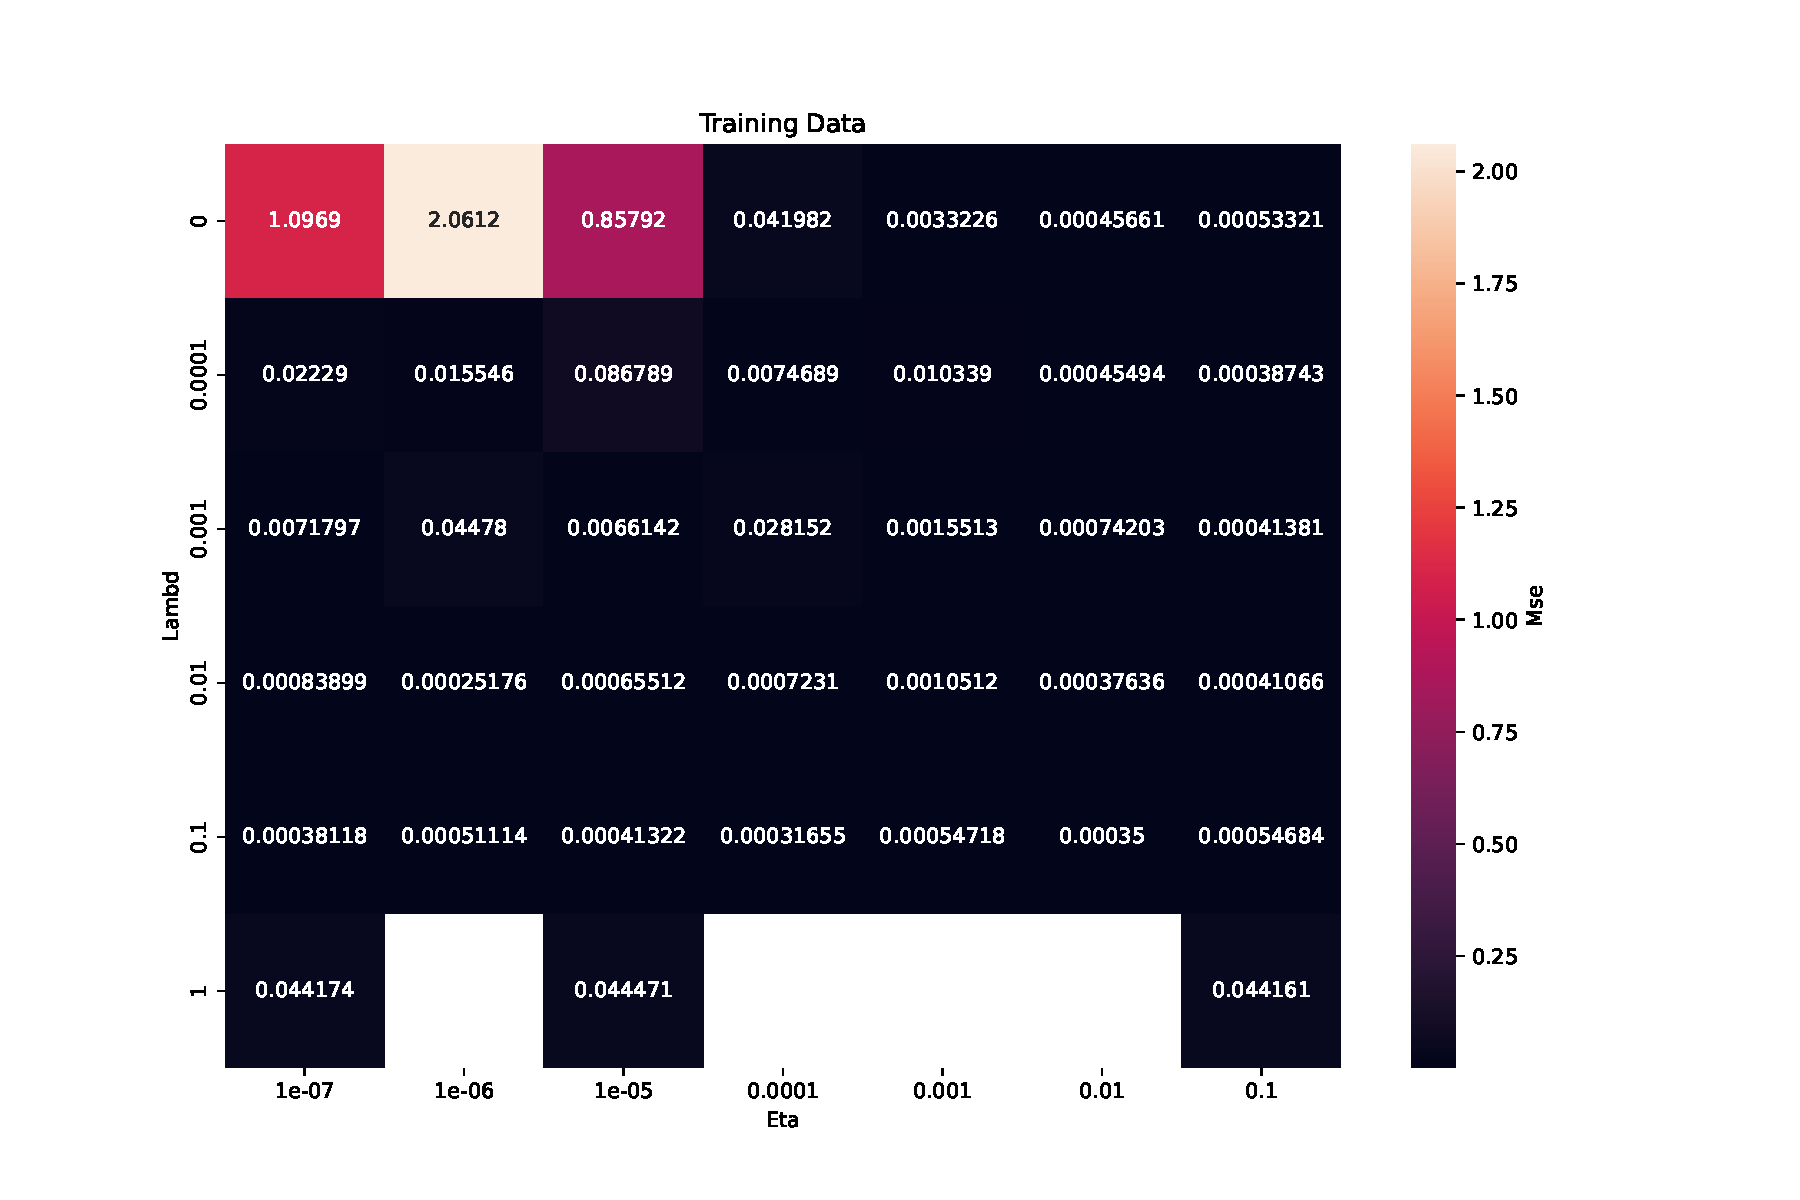
\includegraphics[width=1.1\linewidth]{Figures/PartB/train_leaky_relu_MSE(eta,lmb)}
  \caption{Train MSE}
  \label{fig:train_leaky_relu_MSE-eta-lmb-}
\end{subfigure}%
\begin{subfigure}{.5\textwidth}
  \centering
  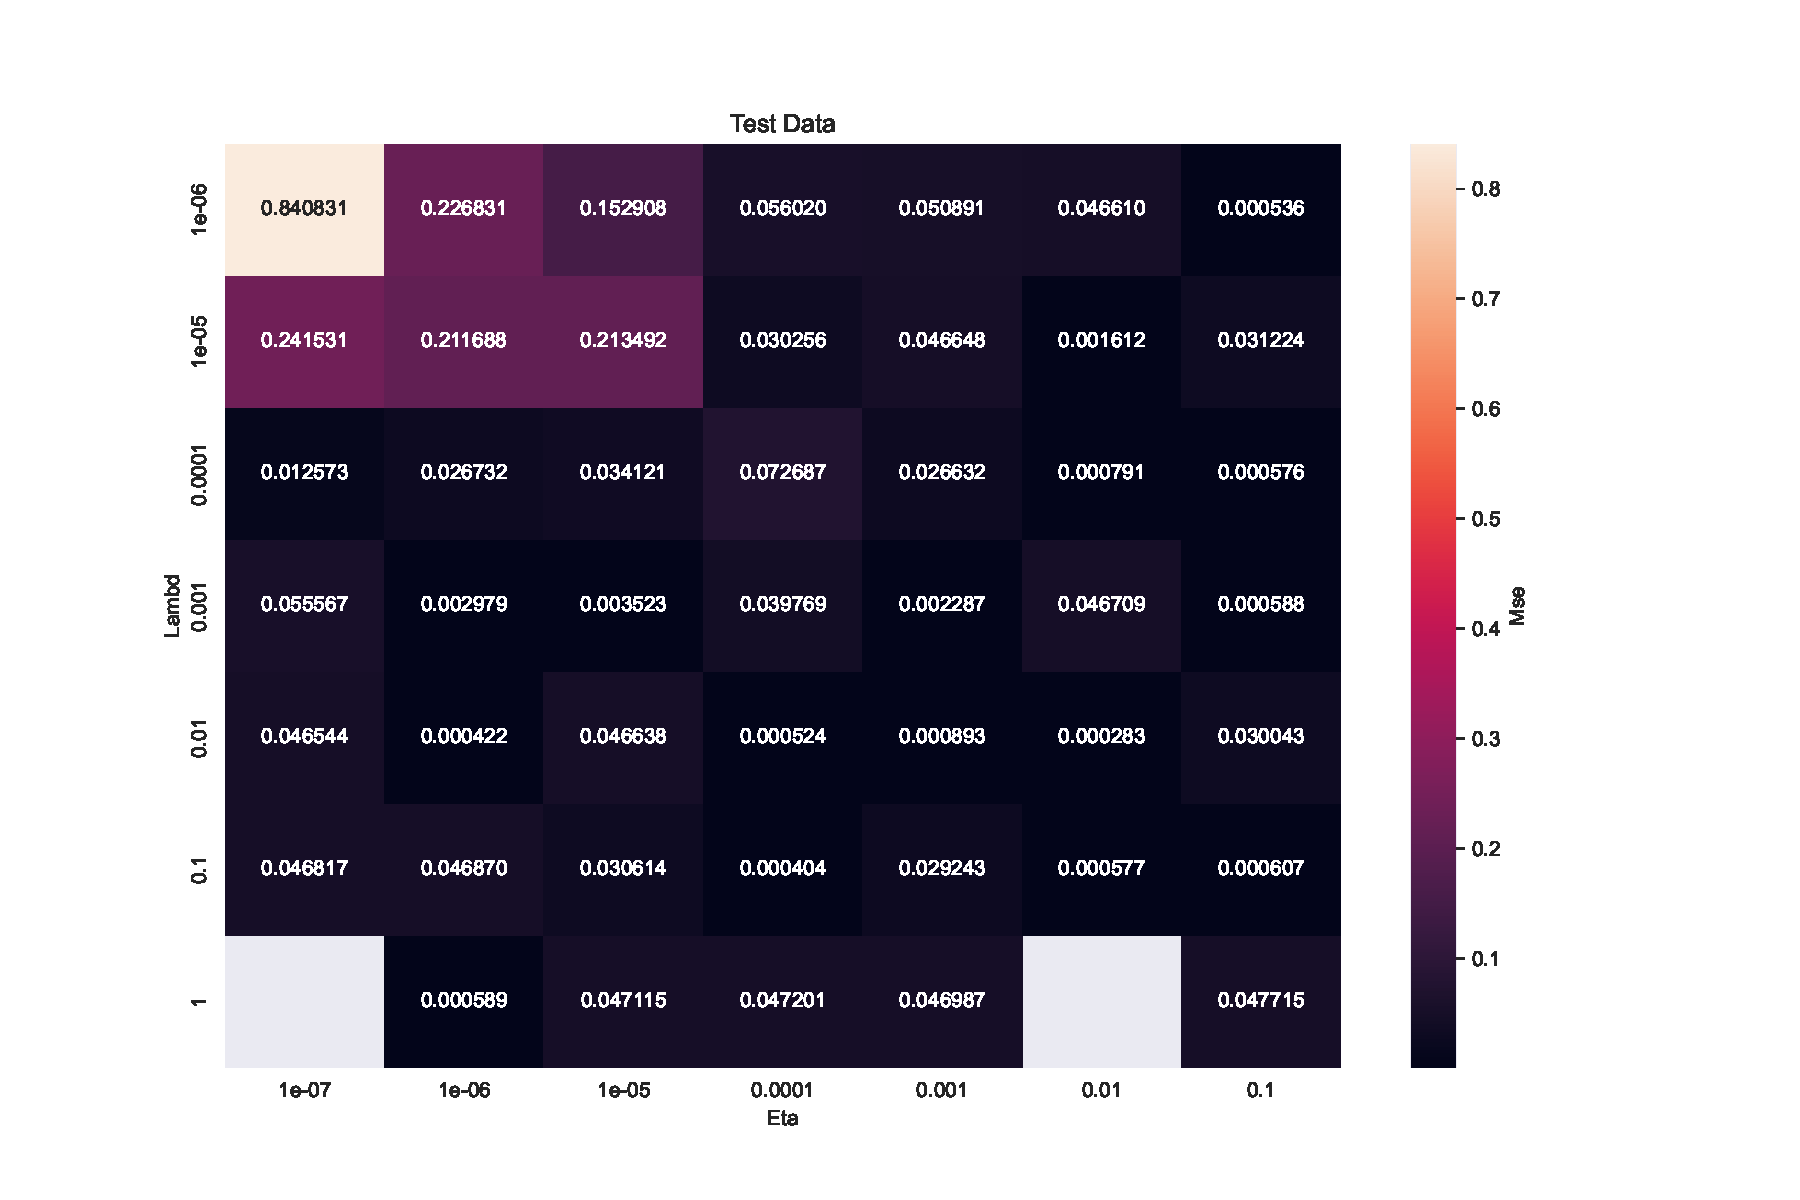
\includegraphics[width=1.1\linewidth]{Figures/PartB/test_leaky_relu_MSE(eta,lmb)}
  \caption{Test MSE}
  \label{fig:test_leaky_relu_MSE-eta-lmb-}
\end{subfigure}
\caption{Neural network with activation function leaky relu: MSE as a function of \(\eta \) and \(\lambda \). 
 The parameters utilized are shown in table \ref{tab:NN_polynomial_parameters2} under run 3.}
\label{fig:leaky_relu_MSE}
\end{figure}

\begin{figure}[htpb]
\begin{subfigure}{.5\textwidth}
  \centering
  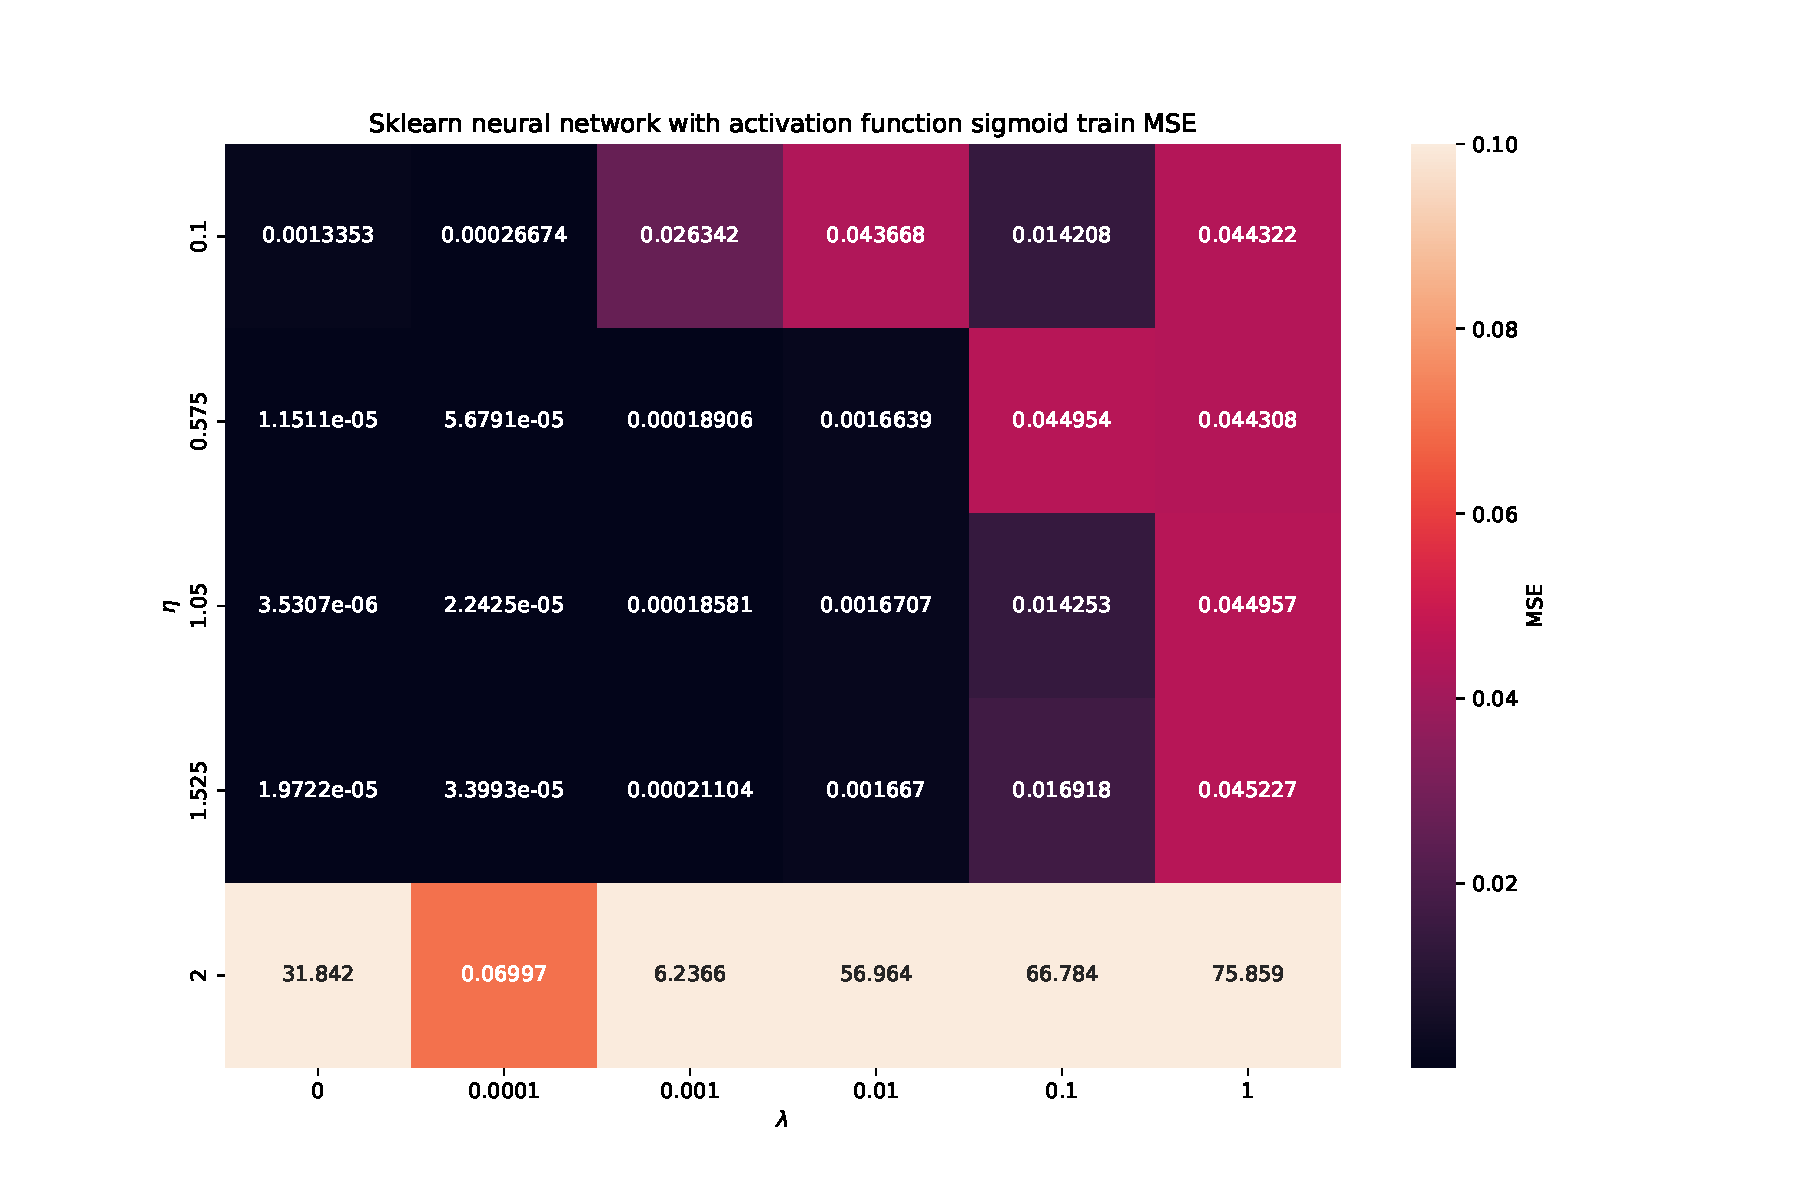
\includegraphics[width=1.1\linewidth]{Figures/PartB/train_sklearn_sigmoid_NN_MSE(eta,lmb)}
  \caption{Sigmoid MSE}
  \label{fig:sklearn_sigmoid_MSE-eta-lmb-}
\end{subfigure}%
\begin{subfigure}{.5\textwidth}
  \centering
  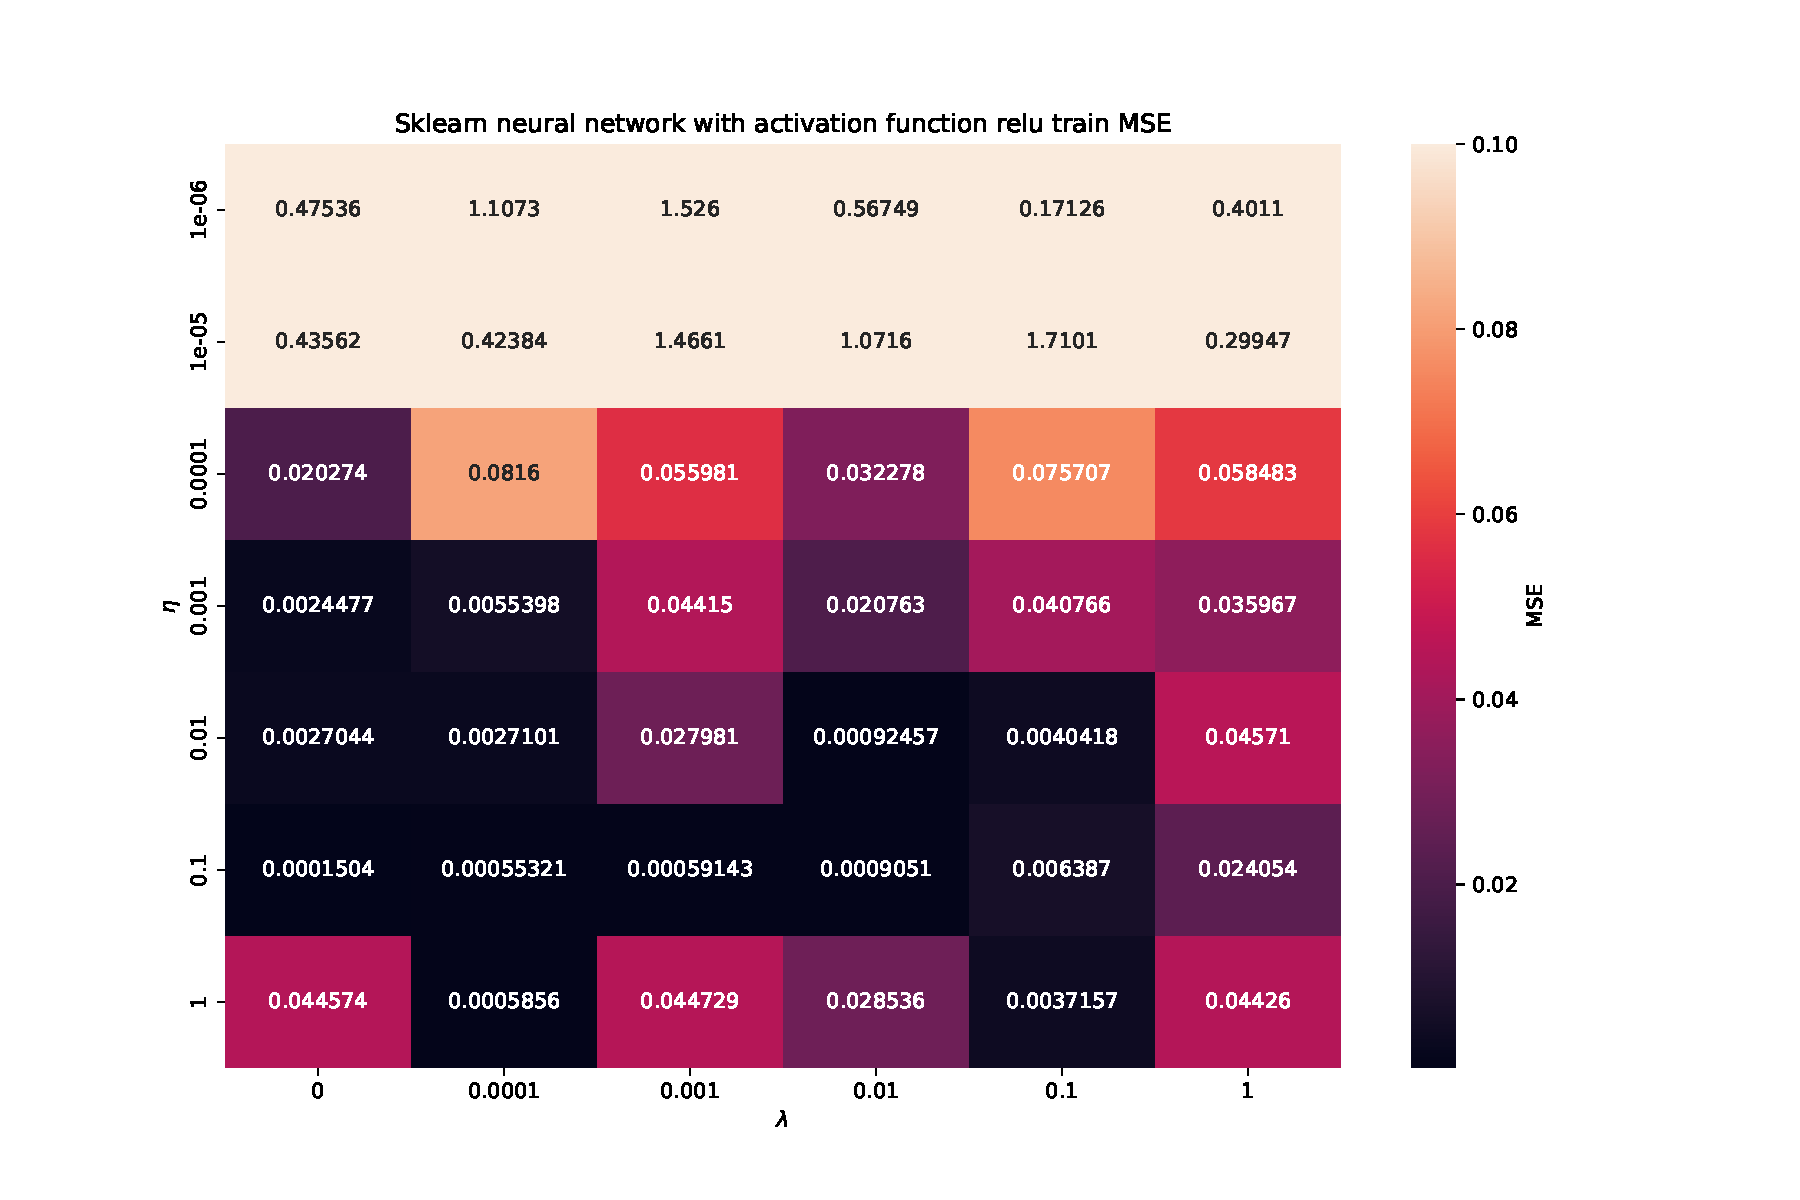
\includegraphics[width=1.1\linewidth]{Figures/PartB/train_sklearn_relu_NN_MSE(eta,lmb)}
  \caption{Relu MSE}
  \label{fig:sklearn_relu_MSE-eta-lmb-}
\end{subfigure}
\caption{SkLearn neural network with activation function sigmoid and relu: Train MSE as a function of \(\eta \) and \(\lambda \).
 The parameters utilized are shown in table \ref{tab:NN_polynomial_parameters2} under run 4 and in table \ref{tab:NN_polynomial_parameters3}
 under run 5 for Sigmoid and ReLU respectively.}
\label{fig:sklearn_MSE}
\end{figure}

Figure \ref{fig:Sigmoid_MSE}-\ref{fig:leaky_relu_MSE} shows training (a) and test (b) MSE for different 
L2-regularzation parameter $\lambda $ (lambd) and differnt learning rates $\eta $ (eta) using activation function Sigmoid, ReLU and leaky 
ReLU on the hidden layer. The same scheme are shown in figure \ref{fig:sklearn_MSE} with activation functions Sigmoid (a) 
and ReLU (b) using \verb|sklearn MLPRegressor|. For sigmoid, we observe that the MSE seems to get stuck around value 0.04
for the larger $\lambda $ and $\eta $ values. %%%%% TODO why?
It is difficult to determine the optimal parameters as no trend is observable other than $\eta $ should be larger than 
$0.0500$ and less than $0.5000$, while $\lambda $ should be less than $0.0100$. The best score was achived with 
$\eta =0.0100$ and $\lambda = 0.3875$ , but every neighboring values are poor suggesting this might just be a lucky run from the 
model's randomness. More runs with different 
random seeds should be analyzed to give more certain answers. 
With ReLU as activation function,the best score was obtained with $\eta =0.1000$ and $\lambda  =0.0001$. There seems to be a trend 
where for smaller $\eta $', larger $\lambda $ is beneficial. The same trend is visible for leaky ReLU where the best score 
was for $\eta= 10^{-6}$ and $\lambda = 0.0100$.

Using activation function sigmoid for the hidden layer gave the best score with $MSE=6.4388 \cdot 10^{-6}$ for the polynomial test data.
Then the next best test score was obtained using ReLU with $MSE=6.9764 \cdot 10^{-5}$, but with less of chance that the network 
gets stuck at training MSE around $0.044$. Leaky ReLU performed worst with a score of $MSE=2.6404 \cdot 10^{-4}$, but it also 
had the least probability of getting stuck. Thus every activation function had its advantages and disadvantages. Comparing 
training and test MSE, we observe that the trained network does not seem to suffer from overfitting.  

Our results seems reasonable by comparing with the results form \verb|sklearn's| neural network, allthough for different learning rates
and \verb|sklearn's| model does not seem to benefit from L2-regularzation. This is because our implementation of the L2-regularization 
parameter was wrong as discussed in section \ref{sec:error_l2_regularization}.

\begin{figure}[H]
\centering
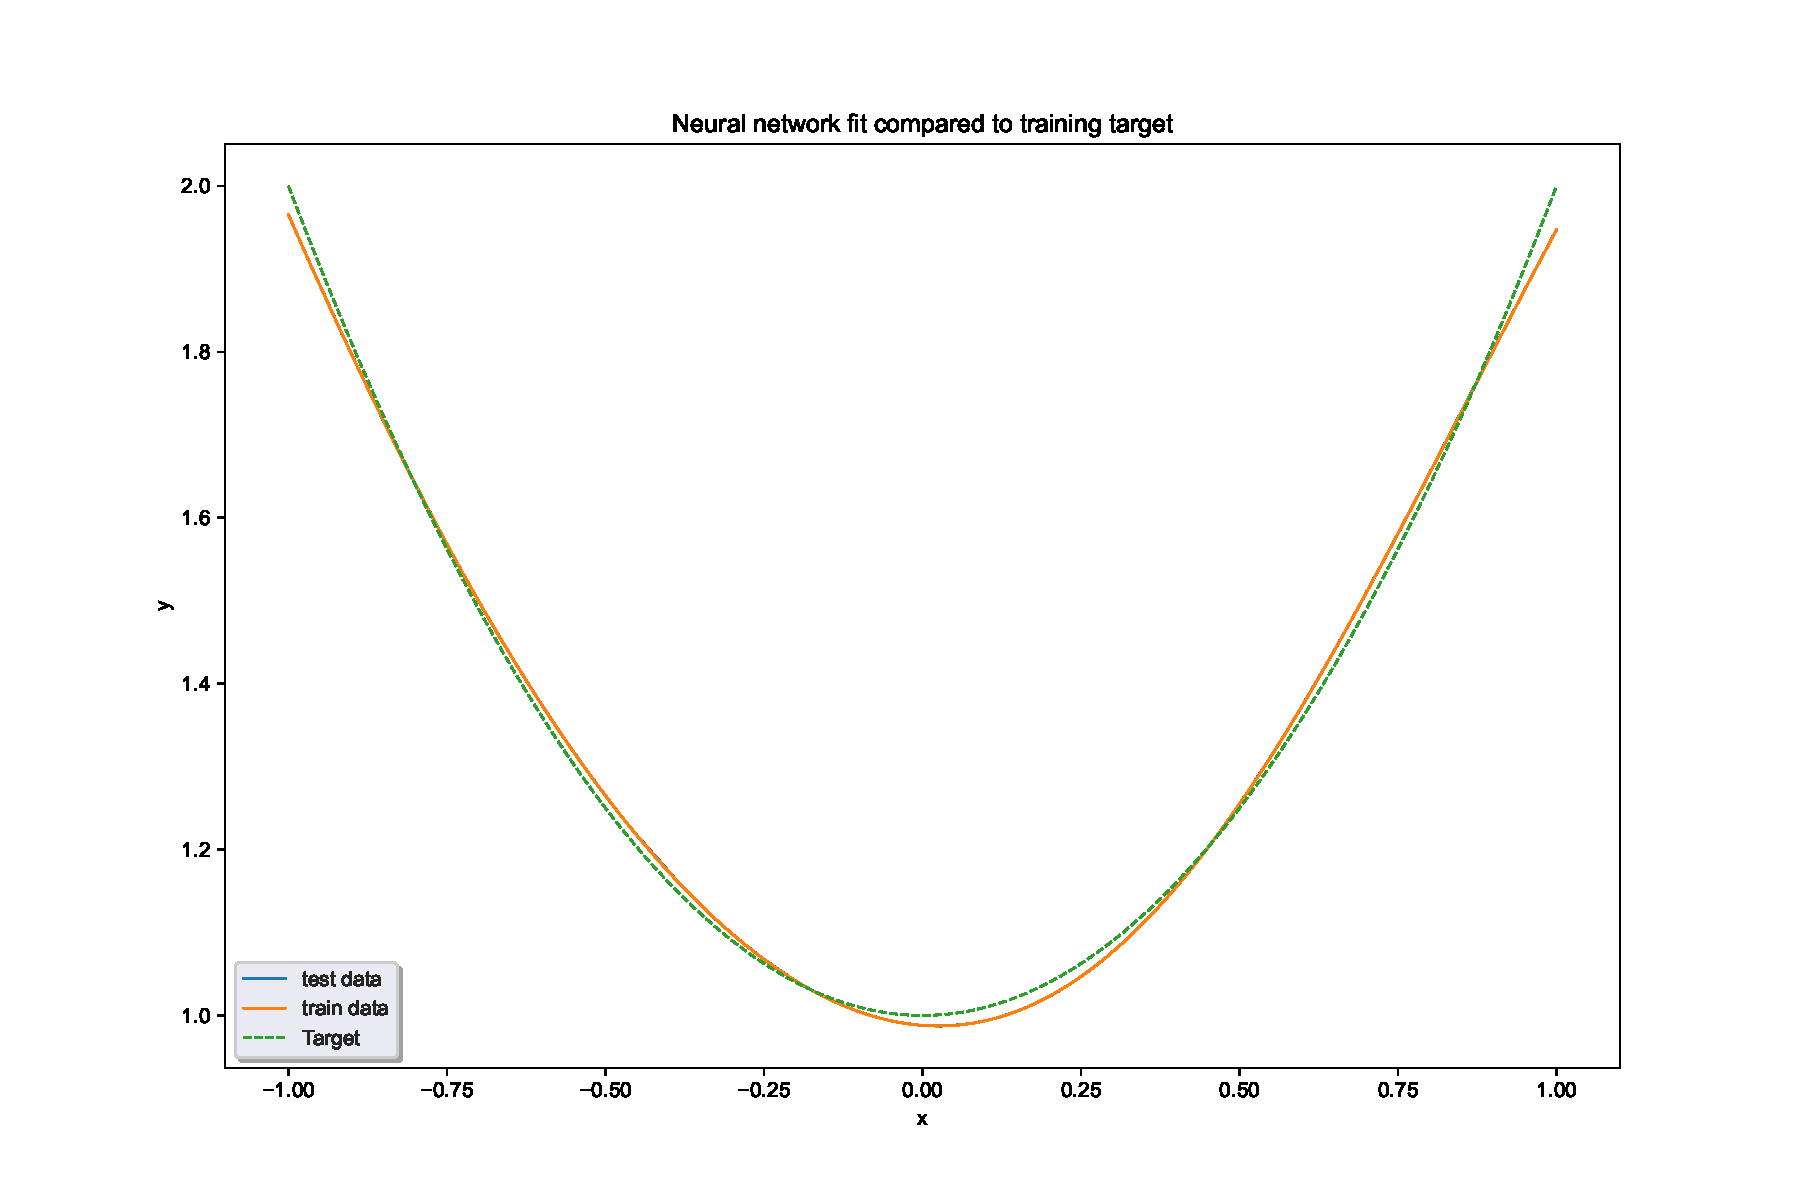
\includegraphics[width=0.8\textwidth]{Figures/PartB/NN_polyfit_result}
\caption{Resulting output after training the neural network with activation function sigmoid compared to the training target. 
The parameters utilized are shown in table \ref{tab:NN_polynomial_parameters3} under run 6.}
\label{fig:NN_polyfit_result}
\end{figure}

Figure \ref{fig:NN_polyfit_result} shows the resulting polynomial fit after training the neural network with activation function Sigmoid. 
Comparing our model to the target, we observe pretty similar shapes allthough we can clearly see some deviation. The polynomial fit obtain 
from gradient descent were much better (which is also obvious comparing MSE), but we have to keep in mind that gradient descent used the second 
order polynomial design matrix such that it was given the information of which order polynomial to optimize (which were the same order as the target poltnomial)
, while the neural network did not have this information. 

